\documentclass{article}
\usepackage[utf8]{inputenc}

% if you need to pass options to natbib, use, e.g.:
% \PassOptionsToPackage{numbers, compress}{natbib}
% before loading nips_2018
\PassOptionsToPackage{square,comma,numbers}{natbib}

% ready for submission
\usepackage{nips_2018}

% to compile a preprint version, e.g., for submission to arXiv, add
% add the [preprint] option:
% \usepackage[preprint]{nips_2018}

% to compile a camera-ready version, add the [final] option, e.g.:
% \usepackage[final]{nips_2018}

% to avoid loading the natbib package, add option nonatbib:
% \usepackage[nonatbib]{nips_2018}

\title{Differentially Private Contextual Linear Bandits}
% \author{
%   Roshan Shariff
%   \And
%   Or Sheffet
% }

\usepackage{newtxtext}
%\usepackage[semibold]{libertine} % a bit lighter than Times--no osf in math
\usepackage[T1]{fontenc} % best for Western European languages
%\usepackage{textcomp} % required to get special symbols
%\usepackage[varqu,varl]{inconsolata} % a typewriter font must be defined
\usepackage{amsmath,mathtools}
\usepackage{amsthm,thmtools,thm-restate}
\usepackage{amssymb} % loads amsfonts
\usepackage{nicefrac}
%\usepackage[libertine,cmintegrals,bigdelims,vvarbb]{newtxmath} %
%replaces some amssymb symbols
\usepackage{newtxmath}
\usepackage[scr=rsfso]{mathalfa} % Use rsfso to provide mathscr
\usepackage{dsfont}
%\usepackage{upgreek}
\usepackage{bm} % load after all math to give access to bold math
\usepackage{etoolbox}

\usepackage{lineno}
\usepackage{microtype}
\usepackage[inline,shortlabels]{enumitem}
\usepackage{setspace}
\usepackage{tikz-cd}
\usepackage{booktabs}
\usepackage{algpseudocode,algorithm}
\usepackage{multicol}
%\usepackage{fullpage}
\usepackage{color}
\usepackage{subcaption}
\newcommand{\os}[1]{\textcolor{red}{Or's comment:~\textbf{#1}}}
%\usepackage{dblfloatfix}

%% Bibliography/References
% \usepackage[round,colon]{natbib}

\bibpunct{\nolinebreak{}[}{]}{,}{n}{}{,}

%% Cross-references
\usepackage{varioref}
\usepackage[pdfusetitle]{hyperref}
% \usepackage{bookmark}
\usepackage[capitalise]{cleveref}

\hypersetup{
  hidelinks,
  bookmarks,
  bookmarksnumbered,
  bookmarksopen,
  bookmarksopenlevel=2
}

%% To-do notes
\usepackage[obeyFinal]{todonotes}

% \newcommand{\tinytodo}[2][]{\todo[size=\tiny]{#2}}
\newcommand{\tinytodo}[2][]{\todo[size=\tiny, #1]{\begin{spacing}{1.0}#2\end{spacing}}}
\newcommand{\RStodo}[2][]{\tinytodo[color=red!20, #1]{R:\@#2}} % Roshan
\newcommand{\OStodo}[2][]{\tinytodo[color=blue!20, #1]{Cs: #2}} % Or
\newcommand{\fix}{\marginpar{FIX}}
\newcommand{\new}{\marginpar{NEW}}

%% Macros

\renewcommand{\vec}[1]{\bm{#1}}
\newcommand{\wildcard}{\mathinner{\,{\cdot}\,}}
\newcommand{\defeq}{\coloneq}
\newcommand{\eqdef}{\eqcolon}
\newcommand{\inv}[1]{#1^{-1}}
\newcommand{\Real}{\mathds{R}}
\newcommand{\Nat}{\mathds{N}}
\newcommand{\Int}{\mathds{Z}}
\newcommand{\mgf}{\mathrm{mgf}}
\newcommand{\UCB}{\mathrm{UCB}}
\newcommand{\ie}{\text{i.e.\@}}
\newcommand{\iid}{\text{i.i.d.\@}}
\renewcommand{\Pr}{\mathds{P}}
\renewcommand\mid{\mathinner{\vert}}
\newcommand{\argmin}{\operatorname*{arg\,min}}
\newcommand{\argmax}{\operatorname*{arg\,max}}
\newcommand{\tr}{\operatorname{tr}}
\newcommand{\rank}{\operatorname{rank}}
\renewcommand{\det}{\operatorname{det}}

\newcommand\given[1][\delimsize]{%
  \providecommand{\delimsize}{}
  \nonscript\:#1\vert\allowbreak\nonscript\:\mathopen{}
}

\DeclarePairedDelimiter{\abs}||
\DeclarePairedDelimiter{\paren}()
\DeclarePairedDelimiter{\brck}{[}{]}
\DeclarePairedDelimiterX{\set}[1]\lbrace\rbrace{#1}
\DeclarePairedDelimiter{\floor}\lfloor\rfloor
\DeclarePairedDelimiter{\ceil}\lceil\rceil
\DeclarePairedDelimiterX{\innerp}[2]\langle\rangle{#1,#2}
\DeclarePairedDelimiterXPP{\Prob}[1]{\Pr}(){}{#1}
\DeclarePairedDelimiterXPP{\PrSet}[1]{\Pr}\{\}{}{#1}
\DeclarePairedDelimiterXPP{\Ex}[1]{\mathds{E}}{[}{]}{}{#1}
\DeclarePairedDelimiterXPP{\Exx}[2]{\mathds{E}_{#1}}{[}{]}{}{#2}
\DeclarePairedDelimiterXPP{\Var}[1]{\mathrm{Var}}{[}{]}{}{#1}
\DeclarePairedDelimiterXPP{\One}[1]{\mathds{1}}\{\}{}{#1}
\DeclarePairedDelimiterXPP{\norm}[2]{}\Vert\Vert{_{#1}}{#2}

%% Other symbols
\newcommand{\A}{\mathcal{A}}
\newcommand{\C}{\mathcal{C}}
\newcommand{\D}{\mathcal{D}}
\newcommand{\E}{\mathcal{E}}
\providecommand\transp{\top}
\let\transpsymbol\transp
\renewcommand{\transp}[1]{#1^\transpsymbol}
\newcommand{\scrF}{\mathscr{F}}
\newcommand{\Wishart}{\mathcal{W}}
\newcommand{\Normal}{\mathcal{N}}
\newcommand{\Eye}[1][]{\bm{I}\notblank{#1}{_{{#1}\times{#1}}}{}}
\newcommand{\XtX}[1]{\transp{#1}{#1}}

\renewcommand{\paragraph}[1]{\vspace{2pt}\noindent\textbf{#1}}
% Theorem environments

\declaretheorem[style=plain]{theorem}
\declaretheorem[style=plain,sibling=theorem]{lemma}
\declaretheorem[style=plain,sibling=theorem]{corollary}
\declaretheorem[style=plain,sibling=theorem]{proposition}
\declaretheorem[style=plain,sibling=theorem]{claim}
\declaretheorem[style=definition,sibling=theorem]{definition}
\declaretheorem[style=definition]{assumption}
\declaretheorem[style=remark]{remark}

\declaretheorem[style=definition,numbered=no]{assumptions}

\newenvironment{assumptions*}[2][]{%
  \begin{assumptions}[#1]
    #2
    \begin{enumerate}[nolistsep]
      \setcounter{enumi}{\theassumption}
      \newcommand{\assume}[1][]{\item\label[assumption]{##1}}
    }{
      \setcounter{assumption}{\theenumi}
    \end{enumerate}
  \end{assumptions}%
}

\Crefname{assumption}{Assumption}{Assumptions}



%%%%%%%%%%%%%%%%%%%%%%%%%%%%%%%%%%%%%%%%%%%%%%%%%%%%%%%%%%%%%%%%%%%%%%%%%%%
%\onehalfspacing

\begin{document}
\setlength{\intextsep}{4pt}
\setlength{\textfloatsep}{4pt}
\setlength{\abovedisplayskip}{3pt}
\setlength{\belowdisplayskip}{3pt}

\maketitle

\begin{abstract}
  We study the contextual linear bandit problem, a version of the
  standard stochastic multi-armed bandit (MAB) problem, where a learner
  sequentially selects actions to maximize a reward which
  depends also on a user provided per-round \emph{context}. Though the context
  is chosen arbitrarily or adversarially, the reward is assumed to
  be a stochastic function of a feature vector that encodes the
  context and selected action. Our goal is to devise private learners for the
  contextual linear bandit problem.

  We first show that using the standard definition of differential
  privacy results in linear regret. So instead, we adopt the notion of \emph{joint}
  differential privacy, where we assume that the action chosen on day
  $t$ is only revealed to user $t$ and thus needn't be kept private
  that day, only on following days. We give a general scheme
  converting the classic linear-UCB algorithm into a joint differentially
  private algorithm using the tree-based algorithm~\cite{ChanPrivateContinualRelease2010,DworkContinualObservation2010}.
  We then apply either Gaussian noise or Wishart noise to acheive joint-differentially private algorithms and bound the resulting algorithms' regrets. In addition, we give the first lower bound on the
  \emph{additional} regret any private algorithms for the MAB problem must incur.
 \end{abstract}

\section{Introduction}
\label{sec:introduction}

The well-known \emph{stochastic multi-armed bandit} (MAB) is a
sequential decision-making task in which a learner repeatedly chooses
an action (or arm) and receives a noisy reward.  The objective is to
maximize cumulative reward by \emph{exploring} the actions to discover
optimal ones (having the best expected reward), balanced with
\emph{exploiting} them.  The \emph{contextual} bandit problem is an
extension of the MAB problem, where the learner also receives a \emph{context} in
each round, and the expected reward depends on \emph{both} the context
and the selected action.

% Since the agent only observes the reward for actions it takes, this
% is an online learning task with partial information.  Learning the
% rewards associated with all the arms requires an agent to
% \emph{explore} them.  Too much exploration, however, would be
% counter-productive; eventually the algorithm should \emph{exploit}
% the best arms it has found.  The main challenge of bandit strategies
% is to balance exploration and exploitation.

As a motivating example, consider online shopping: the user provides a
context (composed of query words, past purchases, etc.), and the site
responds with a suggested product and receives a reward if the user
buys it.  Ignoring the context and modeling the problem as a standard
MAB (with an action for each possible product) suffers from the
drawback of ignoring the variety of users' preferences; whereas separately
learning each user's preferences doesn't allow us to generalize
between users.  Therefore it is common to model the task as a
contextual \emph{linear bandit} problem: Based on the user-given
context, each action is mapped to a feature vector; the
reward probability is then assumed to depend on the \emph{same} unknown linear
function of the feature vector across all users.

The above example motivates the need for privacy in the contextual
bandit setting: users' past purchases and search queries are sensitive personal
information, yet they strongly predict future purchases.
% An algorithm may pick an ad for a
% user based on their own information, and it may even learn from
% aggregated information to choose better in the future, but an
% adversary analyzing these ad choices must not be able to learn too
% much about any individual user.
In this work, we give upper and lower bounds for the
problem of (joint) \emph{differentially private} contextual linear
bandits. Differential privacy is the de facto gold-standard of
privacy-preserving data analysis in both academia and industry,
requiring that an algorithm's output have very limited dependency on
any single user interaction (one context and reward).  However, as we
later illustrate, adhering to the standard notion of differential
privacy (under event-level continual observation) in the contextual bandit
requires us to essentially ignore the context and thus incur linear
regret.  We therefore adopt the more relaxed notion of \emph{joint
  differential privacy}~\citep{KearnsMechanismDesign2014} which,
intuitively, allows us to present the $t$-th user with products
corresponding to her preferences, without revealing (much) about those
preferences to all users at times $t'>t$.\footnote{The guarantee of
  differential privacy under continuous observation assures that 
  even if all later user collude in an effort to learn user $t$'s
  context, they still have very limited advantage over a random
  guess.}

\subsection{Problem Formulation}
\label{subsec:problem_formulation}
\paragraph{Stochastic Contextual Linear Bandits.}
%\label{sec:contextual-bandits}
In the classic MAB problem, in every round $t$ a learner
selects an \emph{action} $a_t$ from a fixed set $\A$ and receives a
\emph{reward} $y_t$.  In the (stationary) \emph{stochastic} MAB, the
reward is noisy with a fixed but unknown expectation
$\Ex{y_t\given a_t}$ that depends only on the selected action.
In the stochastic contextual bandit problem, the learner also receives
a \emph{context} $c_t\in\C$ at the beginning of each round, and the
expected reward $\Ex{y_t\given c_t,a_t}$ depends on both $c_t$ and
$a_t$.  It is common to assume that the context
affects the reward in a linear way: map every context-action pair to a
\emph{feature vector} $\phi(c_t,a_t)\in\Real^d$ (where $\phi$ is an
arbitrary but known function) and assume that
$\Ex{y_t\given c_t,a_t} = \innerp{\vec\theta^*}{\phi(c_t,a_t)}$.  The
vector $\vec\theta^*\in\Real^d$ is the key unknown parameter of the
environment which the learner must discover to maximize reward.
Alternatively, we can assume $\phi$ has been computed already, so each round the learner is given a
%Note how all the learner needs to know about the context is implicitly encoded by the
\emph{decision set}
$\D_t \defeq \set{\phi(c_t,a)\given a\in\A \subset \Real^d}$, where
choosing $x_t\in\D_t$ effectively determines the action
$a_t\in\A_t$.  Thus, the contextual stochastic linear bandit framework
consists of repeated rounds in which the learner
\begin{enumerate*}[(i),before=\unskip{: },itemjoin={{; }},itemjoin*={{; and }}]
\item receives a \emph{decision set} $\mathcal{D}_t \subset \Real^d$
\item chooses an \emph{action} $\vec x_t \in \mathcal{D}_t$
\item receives a stochastic \emph{reward}
  $y_t = \innerp{\vec\theta^*}{\vec x_t} + \eta_t$.
\end{enumerate*}
When all $\D_t$s are identical (and have orthogonal vectors) the problem reduces to standard MAB.

The learner's objective is to maximize cumulative reward, which is equivalent to
minimizing \emph{regret} --- the extra reward a
learner would have received by always choosing the best available
action.
%An effective learner may nevertheless earn only a small reward if all the actions are poor, but would then still achieve low regret.
In other words, the regret characterizes the cost of having
to \emph{learn} the optimal action over just \emph{knowing} it beforehand.
For stochastic problems, we are usually interested in a related
quantity called \emph{pseudo-regret}, which is the extra
\emph{expected} reward that could have been earned had the learner known $\vec\theta^*$ in advance.  In our setting,
the cumulative pseudo-regret after $n$ rounds is
$\widehat{R}_n \defeq
\sum_{t=1}^n\max_{x\in\D_t}\innerp{\vec\theta^*}{\vec x - \vec x_t}$.%
\footnote{The pseudo-regret ignores the reward noise but not the
  randomness in the learner's choice of actions.  It equals the reward
  in expectation, but is more amenable to high-probability bounds such
  as those we provide. In particular, in some cases we can acheive polylog$(n)$ pseudo-regret bounds because pseudo-regret isn't masked by the
  unavoidable reward noise, whose standard-deviation is $\Omega(\sqrt n)$.}


\paragraph{Joint Differential Privacy.} %
%\label{sec:joint-dp}
As discussed above, the context and reward may be considered private
information about the users which we wish to keep private from all
\emph{other} users. We thus introduce the notion of joint
differentially private learners under continuous observation, a
combination of two definitions \citep[given
in][]{KearnsMechanismDesign2014,DworkContinualObservation2010}. First,
we say two sequences
$S = \langle (\mathcal{D}_1, y_1), (\mathcal{D}_2, y_2), ...,
(\mathcal{D}_n, y_n) \rangle$ and
$S' = \langle (\mathcal{D}'_1, y'_1), ..., (\mathcal{D}'_n, y'_n)
\rangle$ are \emph{$t$-neighbors} if for all $t'\neq t$ it holds that
$(\mathcal{D}_{t'},y_{t'}) = (\mathcal{D}'_{t'}, y'_{t'})$.
%\os{maybe omit?} We say $S$ and $S'$ are \emph{neighbors} if there exists a $t$ such that the two sequences are $t$-neighbors.
% For example, a
% search engine might have a context consisting of a user's search
% query, identity, interests, and physical location, while the reward
% indicates which search result the user clicked on.  The search engine
% should, of course, use the context to answer each query; furthermore,
% it should learn from the reward to better respond to future queries
% from other users.  However, it should also maintain privacy: its
% responses to queries should not reveal \emph{too much} information
% about the context and rewards it has learned from.  More precisely, we
% want algorithms that are \emph{jointly differentially private} in the
% following sense:

\begin{definition}
\label{def:joint-dp}
  A randomized algorithm $A$ for the contextual bandit problem is
  \emph{$(\varepsilon,\delta)$-jointly differentially private} (JDP) under continual observation if for any $t$ and any pair of $t$-neighboring sequences $S$ and $S'$, and any subset ${\cal S}_{>t} \subset \mathcal{D}_{t+1} \times \mathcal{D}_{t+2} \times \cdots \times \mathcal{D}_{n}$ of sequence of actions ranging from day $t+1$ to the end of the sequence, it holds that $\Pr[A(S)\in \mathcal{S}_{>t}] \leq e^\varepsilon\Pr[A(S')\in \mathcal{S}'_{>t}] +\delta$.
\end{definition}
Note that the standard definition of differential privacy requires the
distribution proximity to hold for any subset of sequences of actions
ranging from day $t$ to the end of sequence. However, in our problem
formulation, with given decision sets, this notion isn't even
well-defined --- the decision set of day $t$ is different under $S$
and under $S'$. Therefore, when we discuss the impossibility of
regret-minimization under standard differential privacy, we revert
back to the setting of different contexts with fixed action set. See
\cref{sec:lower_bounds} for further details.

\subsection{Our Contribution and Paper Organization}
\label{subsec:contributions}

In this work, in addition to formulating the definition of JDP under
continual observation, we also present a framework for implementing
JDP algorithms for the contextual bandit problem. Not surprisingly,
our framework combines the tree-based algorithm~\cite{ChanPrivateContinualRelease2010,DworkContinualObservation2010}  with the linear
upper-confidence bound (LinUCB) algorithm~\cite{DaniStochasticLinearOptimization2008}.  However, for modularity,
in Section~\ref{sec:LinUCB} we first analyze a family of linear UCB algorithms where in each
day one uses a different regularizer, under the premise that all
regularizers' singular values are bounded. Moreover, we repeat our analysis twice. Once in a general framework,
obtaining an upper bound on the regret which is proportional to
$\tilde O(\sqrt n)$; and once in an instance dependent setting, where in each
day there's a significant gap of at least $\Delta$ between the best arm and any other
arms, obtaining a regret upper bound of $\mathrm{polylog}(n)/\Delta$.
% \footnote{The analysis carries through to $k-1$ gaps between the $i$th
% arm and the leading one, yet its result is too cumbersome so we omit
% this analysis.} 
Our leading application of course is privacy, though
one could postulate other reasons why such a change in regularizers
would be useful (e.g., updating the regularizer when an initial upper
bound of a parameter turns out to be wrong). We then plug-in two
particular regularizers into our scheme: one based on additive Wishart
noise~\citep{SheffetPrivateApproxRegression2015} which always results
in a PSD matrix, achieving regret of $\tilde O(\sqrt{n}(d+\nicefrac{\sqrt d}{\varepsilon}))$; and one based on additive Gaussian
noise \citep{DworkAnalyzeGauss2014} shifted by $\Upsilon\Eye$ to make
it PSD w.h.p.\ over all days, giving a regret bound of $\tilde O(\sqrt n d/\varepsilon)$. (The actual bounds depends on \emph{many} variables, so there are settings where the latter is better than the former.) The details of the two techniques are given in Section~\ref{sec:alg-dp}.
%We also present empirical evidence showing our analysis is in fact optimal, presented in Section~\ref{}.

In Section~\ref{sec:lower_bounds} we also give a lower bound for the $\varepsilon$-differentially private
MAB problem. Whereas all previous work on the private MAB problem uses standard (non-private) bounds, we show that
\emph{any} private algorithm must incur \emph{an additional} regret of
$\Omega(k\log(n)/\varepsilon)$. While the result resembles the lower bound in the
adversarial setting, the proof technique cannot rely on standard packing arguments~\citep[e.g.][]{HardtTalwarGeometryDP2010} since the input for the
problem is stochastic rather than adversarial.  Instead, we rely on a recent coupling argument given in~\cite{KarwaVadhanFiniteSampleDP2017} to prove any private algorithm must substantially explore suboptimal arms.

\paragraph{Future Directions.} The linear-UCB algorithm we adapt in this work is a canonical approach to the linear MAB problem, also referred to as ``optimism in the face of uncertainty.'' However, a recent work~\cite{LattimoreS17} shows that in certain situations it is best to adjust to the actions in the decision set in a very particular way, that utilizes a complicated optimization problem. We pose here the question of devising a private version of the algorithm in~\cite{LattimoreS17} which interpolates between UCB and fine-tuning to the specific action set. 
\vspace{-0.5mm}
\subsection{Related Work}
\label{subsec:related_work}
%\paragraph{MAB and the Contextual Bandit Problem.}
The MAB dates to the seminal work of Robbins~\cite{robbins1952}, with the UCB approach developed in a series of works~\cite{BanditBook85,Agrawal95} culminating in~\cite{Auer2002}.  Stochastic linear bandits were formally first introduced in~\cite{Abe2003}, and~\cite{Auer2003UCB} was the first paper to consider UCB-style algorithms. An algorithm that is based on a confidence ellipsoid is described in~\cite{DaniStochasticLinearOptimization2008}, with a variant based on ridge regression given in~\cite{ChuLRS11}, or explore-then-commit variant in~\cite{RusmevichientongT10}, and a variant related to a sparse setting appears in~\cite{Abbasi-YadkoriPS12}. \cite{AbbasiYadkoriImprovedAlgorithmsLinear2011} gives an instance dependent bound for linear bandits, which we convert to the contextual setting.
%\todo[inline]{Complete this section.}


%\paragraph{Differential Privacy.}
Differential privacy, first introduced by
\citet{DworkCalibratingNoiseSensitivity2006,DworkOurData2006}, is a
rigorous mathematical notion of privacy that requires the probability
of any observable output to change very little when any single datum
changes.  (We omit the formal definition because we already defined JDP.)
%A classic result~\cite{DworkOurData2006} states that if $f$ is a function of the input whose $L_2$-norm cannot change by more than $B$ with a change of a single datum, then adding Gaussian noise to $f$ of $0$-mean and variance $B^2\log(\nicefrac 1 \delta)/\varepsilon^2$ preserves $(\varepsilon,\delta)$-differential privacy.
Among its many elegant traits is the notion of group privacy: should
$k$ datums change then the change in the probability of any event is
still limited by (roughly) $k$ times the change when a single datum
was changed.  A different property of differential privacy is composition~\cite{DworkBoosting2010}: The combination of $k$ $(\varepsilon,\delta)$-differentially private algorithms is $\paren[\big]{O(k\varepsilon^2 + 2\sqrt{k\log(\nicefrac 1 {\delta'})}), k\delta+\delta'}$-differentially private for any $\delta'>0$.
%
The notion of differential privacy under continual observation was
first defined by \citet{DworkContinualObservation2010} using the \textbf{tree-based algorithm}~\citep[originally
appearing in][]{ChanPrivateContinualRelease2010}. This algorithm
maintains a binary tree whose $n$ leaves correspond to the $n$ entries
in the input sequence. Each node in the tree maintains a noisy
(privacy-preserving) count of the sum of the input entries in its
subtree, thus enabling us to maintain a running count of the sum of
inputs by combining at most $\log(n)$ noisy counts. This
algorithm is the key ingredient of a variety of works that deal with
privacy in an online setting, including
counts~\cite{DworkContinualObservation2010}, online convex
optimization~\cite{JainDPOnlineLearning2012}, and regret minimization
in both the
adversarial~\citep{SmithThakurtaPrivateOnlineLearning2013,TossouAchievingPrivacyAdversarial2017}
and
stochastic~\cite{MishraNearlyOptimalDPBandits2015,TossouAlgDPBandits2016}
settings. We comment that \citet{MishraNearlyOptimalDPBandits2015}
proposed an algorithm similar to our own for the contextual bandit
setting, however (i)~without maintaining PSD, (ii)~without any
analysis, only empirical evidence, and (iii)~without presenting lower
bounds. Further details about acheiving differential privacy via additive noise and the tree-based algorithm appear in Section~\ref{apx_sec:more_background} of the supplementary material.
%
The related problem of private linear regression have also been extensively studied in the offline setting
\citep{ChaudhuriDPERM2011,BassilyPrivateEmpiricalRisk2014}.

\section{Preliminaries and Notation}
\label{sec:preliminaries}

We use $\vec{bold}$ character to denote vectors and bold
$\vec{CAPITAL}$ letters to denote matrices. 
Given a $d$-column matrix
$\vec M$, its \emph{Gram matrix} is the $(d\times d)$-matrix
$\transp{\vec M}\vec M$.  A matrix $\vec M$ is positive-semidefinite
(PSD), denoted $M\succeq 0$ if for any $\vec x$ it holds that
$\transp{\vec x} \vec M \vec x \geq 0$.  We use $\vec M\succeq \vec N$
to denote the fact that $(\vec M-\vec N)$ is PSD; any such $\vec M$
defines an inner product between vectors, so we define
$\norm{M}{x} = \transp{\vec x} \vec M \vec x$.  The
Gaussian distribution $\Normal(\mu,\sigma^2)$ is defined by the density
function
$(2\pi\sigma^2)^{-0.5}\exp(-\nicefrac{(x-\mu)^2}{2\sigma^2})$. The
$L_2$-norm squared of a $d$-dimensional vector whose coordinates are
drawn iid from $\Normal(0,1)$ is given by the $\chi^2$-distribution,
which is tightly concentrated around $d$. Given two distributions $P$
and $Q$ we denote their \emph{total variation} distances as
$d_{\rm TV}(P,Q) = \max_{{\rm
    event}~E}|\Pr_P[E]-\Pr_Q[E]|$.  %Explicit concentration bounds are given in Section~\ref{}

\paragraph{Notation.}\label{sec:notation} Our bound depends on many
parameters of the problem, specified below. Additional parameters
(bounds) are specified in the assumptions stated below.
\setlength{\multicolsep}{4.0pt plus 2.0pt minus 1.5pt}
\begin{multicols}{2}[]
  \nolinenumbers
  \begin{description}[style=sameline,leftmargin=2em,nosep]
  \item[$n$] horizon, i.e. number of rounds
  \item[$s,t$] indices of rounds
  \item[$d$] dimensionality of action space
  \item[$\D_t$] $\subset\Real^d$; decision set at round $t$
  \item[$\vec x_t$] $\in \D_t$; action at round $t$ \todo{Is this necessary? It was specified in the problem definition. Can it be merged with 6?}
  \item[$y_t$] $\in \Real$; reward at round $t$
  \item[$\vec\theta^*$] unknown parameter vector in $\Real^d$
  \item[$m$] $\defeq \lceil\log_2(n)+1 \rceil$
  \item[$\vec X_{<t}$] $(t-1)\times d$ matrix with $\vec X_{<t,s} = \transp{\vec
      x_s}$ for $s<t$
  \item[$\vec G_t$] Gram matrix of the actions: $\XtX{\vec X_{<t}}$
  \item[$\vec H_t$] regularizer at day $t$
  \item[$\vec y_{<t}$] vector of rewards up to day $t-1$
  \item[$\vec u_t$] action-reward product: $\transp{\vec X_{<t}} \vec y_{<t}$
  \item[$\vec h_t$] perturbation of $\vec u_t$
  %\item[$\norm{V}{\vec x}$] $\defeq \sqrt{\transp{\vec x} V \vec x}$
%   \item[$L$] a bound on the norm of all actions (in all rounds)
%   \item[$B$] a bound on the mean of the rewards: $|\langle \vec x,\vec\theta^*\rangle| \leq B$.
% \item[$\tilde B$] a bound on the reward itself.
% \item[$\tilde L$] $\defeq \sqrt{L^2+\tilde B^2}$.
  \end{description}
  \linenumbers
\end{multicols}
\section{Linear UCB with Changing Regularizers}
\label{sec:LinUCB}

%Our differentially private contextual linear bandit algorithm is based on
In this section we introduce and analyze a variation of
the well-studied LinUCB algorithm, an application of the Upper
Confidence Bound (UCB) idea to stochastic linear bandits
\citep{DaniStochasticLinearOptimization2008,RusmevichientongLinearlyParameterizedBandits2010,AbbasiYadkoriImprovedAlgorithmsLinear2011}.
At every round $t$, LinUCB constructs a \emph{confidence set} $\E_t$
that contains  with high probability the unknown parameter vector $\vec\theta^*$.  It then computes an upper confidence bound on the reward
of each action in the decision set $\D_t$, and ``optimistically''
chooses the action with the highest UCB:
$\vec x_t \gets \argmax_{\vec x\in\D_t} \UCB_t(\vec x)$, where
$\UCB_t(\vec x) \defeq \max_{\vec\theta\in\E_t}
\innerp{\vec\theta}{\vec x}$.  We assume the rewards are linear with
added subgaussian noise (i.e.,
$y_s = \innerp{\vec\theta^*}{\vec x_s} + \eta_s$ for $s<t$), so it is
natural to center the confidence set $\E_t$ on the (regularized)
linear regression estimate:
\begin{align*}
  \hat{\vec\theta}_t
  &\defeq \min_{\hat{\vec\theta} \in \Real^d} \norm{}{\vec X_{<t} \hat{\vec\theta}
    - \vec y_{<t}}^2 + \norm{\vec H_t}{\hat{\vec\theta}}^2
    = \inv{(\vec G_t + \vec H_t)} \transp{\vec X_{<t}} \vec y_{<t}.
    &\text{where } \vec G_t \defeq \XtX{\vec X_{<t}}
\end{align*}
The matrix $\vec V_t \defeq \vec G_t + \vec H_t \in \Real^{d\times d}$ is a regularized
version of the Gram matrix $\vec G_t$.  Whenever the learner chooses an
action vector $\vec x\in \D_t$, the corresponding reward gives it some information
about the projection of $\vec\theta^*$ onto $\vec x$.  In other
words, the estimate $\hat{\vec\theta}$ is probably closer to
$\vec\theta^*$ along the directions where many actions have
been taken.  This motivates the use of ellipsoidal confidence sets
that are smaller in such directions, inversely
corresponding to the eigenvalues of $\vec G_t$ (or $\vec V_t$). The ellipsoid
is uniformly scaled by $\beta_t$ to achieve the desired confidence
level, as prescribed by \cref{prop:calc-beta}.
\begin{align}\label{eq:def-ellip}
  \E_t &\defeq \set{\vec\theta\in\Real^d \given
        \norm{\vec V_t}{\vec\theta-\hat{\vec\theta}_t} \le \beta_t},
  &\text{ for which }
    \UCB_t(\vec x) &= \innerp{\hat{\vec\theta}}{\vec x} + \beta_t\norm{\inv{\vec V_t}}{\vec x}.
\end{align}
Just as the changing regularizer $\vec H_t$ perturbs the Gram matrix $\vec G_t$,
our algorithm allows for the vector
$\vec u_t \defeq \transp{\vec X_{<t}} \vec y_{<t}$ to be perturbed
by $\vec h_t$ to get
$\tilde{\vec u}_t \defeq \vec u_t + \vec h_t$.  The estimate
$\hat{\vec\theta}_t$ is replaced by
$\tilde{\vec\theta}_t \defeq \inv{\vec V_t}\tilde{\vec u}_t$.

\begin{algorithm}[h]
  \caption{Linear UCB with Changing Perturbations}\label{alg:linucb}
  \begin{algorithmic}
    \State \textbf{Initialize:} $\vec G_1 \gets \vec 0_{d\times d}$,
    $u_1\gets \vec 0_{d}$.
    \For{each round $t = 1,2,\dotsc,n$}
    \State Receive $\D_t \gets{}$ decision set ${} \subset \Real^d$.
    \State Receive regularized $\vec V_t \gets \vec G_t + \vec H_t$ and perturbed $\tilde{\vec u}_t \gets \vec u_t + \vec h_t$
    \State Compute regressor $\tilde{\vec\theta}_{t} \gets \inv{\vec V_{t}}\tilde{\vec u}_{t}$
    \State Compute confidence-set bound $\beta_t$ based on Porposition~\ref{prop:calc-beta}.
    \State Pick action $\vec x_t \gets \argmax_{\vec x\in\D_t}
    \innerp{\tilde{\vec \theta}_t}{\vec x} +
    \beta_t\norm{\inv{\vec V_t}}{\vec x}$.
    %\Comment{Choose action.}
    \State Observe $y_t \gets {}$ reward for action $\vec x_t$
    %\Comment{Observe reward.}
    \State Update: $\vec G_{t+1} \gets \vec G_{t} + \vec x_t \transp{\vec x_t},
    \quad \vec u_{t+1} \gets \vec u_{t} + \vec x_t y_t$
    %\Comment{Record in privacy-preserving history.}
    \EndFor
  \end{algorithmic}
\end{algorithm}

Our analysis relies the following assumptions about the environment
and algorithm:
\begin{assumptions*}[\Cref{alg:linucb}]{%
    For all rounds $t=1,\dotsc,n$ and actions $\vec x\in\D_t$:}
  \assume[ass:x-bound] Bounded action set: $\norm{}{\vec x} \le L$.
  \assume[ass:meanreward-bound] Bounded \emph{mean} reward:
  $\abs{\innerp{\vec\theta^*}{\vec x}} \le B$ with $B\ge 1$.%
  \footnote{See \cref{remark:meanreward-bound} preceding the proof of
    \cref{lemma:linucb-regret} in \cref{sec:more-linucb-discussion} of
    the supplementary material for a discussion as to bounding $B$ by $1$ from below.} %
  \assume[ass:thetastar-bound] Bounded target parameter:
  $\norm{}{\vec\theta^*} \le S$.  \assume[ass:psd-reg] All
  regularizers are PSD $\vec H_t \succeq 0$.  \assume[ass:subgaussian]
  $y_t = \innerp{\vec\theta^*}{\vec x_t} + \eta_t$ where $\eta_t$ is
  $\sigma^2$-conditionally subgaussian on previous actions and
  rewards, i.e.:
  %\begin{align*}
    $\Ex{\exp(\lambda\eta_t) \given \vec x_1, y_1, \dotsc, \vec x_{t-1}, y_{t-1}, \vec x_t}
    \le \exp(\lambda^2\sigma^2/2)$, for all $\lambda\in\Real$.
  %\end{align*}
  \assume[ass:bounded-data]
  Strongest bound on both the action and the reward:
  $\norm{}{\vec x_t}^2 + y_t^2 \le \tilde L^2$ for all rounds $t$.  In
  particular, if $\norm{}{\vec x_t} \le L$ (\cref{ass:x-bound}) and
  the rewards are bounded: $\abs{y_t} \le \tilde B$ (not just their
  means as in \cref{ass:meanreward-bound}), we can set $\tilde L^2 = L^2 + \tilde B^2$.
\end{assumptions*}

\cref{ass:x-bound,ass:meanreward-bound} aren't required to have good pseudo-regret bounds, they merely simplify the bounds on the confidence set (see Proposition~\ref{prop:calc-beta} and Section~\ref{sec:regret-bounds}). \cref{ass:bounded-data} is not required at all for now, it is only used for joint-differential privacy in Section~\ref{sec:alg-dp}.


% \cref{ass:x-bound,ass:meanreward-bound} are not needed for the
% correctness of the algorithm (i.e.\ its confidence sets), only for the
% regret bounds in \cref{sec:regret-bounds}.  Conversely, it is
% important to note that of these, only \cref{ass:x-bound} is needed for
% differential privacy (see \cref{ass:bounded-data} in \cref{sec:alg-dp}).

To fully describe Algorithm~\ref{alg:linucb} we need to specify how to compute the confidence-set bounds $(\beta_t)_t$. On the one hand, these bounds have to be accuracte~--- the confidence set $\E_t$ should contain the unknown $\vec\theta^*$; on the other hand, the larger they are, the larger the regret bounds we obtain. 
In other words, the $\beta_t$ should be as small as possible subject to being accurate.

\begin{definition}[Accurate $(\beta_t)_t$]\label{def:accurate-beta}
  A sequence $(\beta_t)_{t=1}^n$ is $(\alpha, n)$-\emph{accurate} for
  $(\vec H_t)_{t=1}^n$ and $(\vec h_t)_{t=1}^n$ if, with probability at
  least $1-\alpha$, it satisfies
  $\norm{\vec V_t}{\vec\theta^* - \tilde{\vec\theta}_t} \le \beta_t$
  for all rounds $t=1,\dotsc,n$ simultaneously.
\end{definition}

We now argue that 3 parameters are the key to establishing accurate confidence-set bounds $(\beta_t)_{t=1}^n$~--- taking into account the noise in the setting \emph{and} the noise added by a changing $\vec H_t$ and $\vec h_t$.

\begin{definition}[Accurate $\rho_{\min}$, $\rho_{\max}$, and
  $\gamma$]\label{def:accurate-params}
  The bounds $0 < \rho_{\min} \le \rho_{\max}$ and $\gamma$ are
  $(\alpha/2n)$-\emph{accurate} for $(\vec H_t)_{t=1}^n$ and $(\vec h_t)_{t=1}^n$ if for a given $t$ w.p. $\leq \alpha/2n$ any of the following does not hold
  \begin{align*}
    \norm{}{\vec H_t} &\le \rho_{\max},
    &\norm{}{\inv{\vec H_t}} &\le \nicefrac{1}{\rho_{\min}},
    &\norm{\inv{\vec H_t}}{\vec h_t} &\le \gamma.
  \end{align*}
\end{definition}

\begin{restatable}[Calculating $\beta_t$]{proposition}{CalcBeta}%
  \label{prop:calc-beta}
  Suppose
  \cref{ass:thetastar-bound,ass:psd-reg,ass:subgaussian}
  hold and let $\rho_{\min}$, $\rho_{\max}$, and $\gamma$ be
  $(\alpha/2n)$-accurate for some $\alpha\in(0,1)$ and horizon $n$.
  Then $(\beta_t)_{t=1}^n$ is $(\alpha,n)$-accurate where
  \begin{align*}
    \beta_t
    &\defeq \sigma\sqrt{2\log(2/\alpha) + \log(\det \vec V_t) - d\log(\rho_{\min})}
      + S\sqrt{\rho_{\max}} + \gamma \\
    &\le \sigma\sqrt{2\log({2}/{\alpha}) + d\log\paren[\Big]{\tfrac{\rho_{\max}}{\rho_{\min}}
      + \tfrac{tL^2}{d\rho_{\min}}}}
      + S\sqrt{\rho_{\max}} + \gamma.
    &\text{(if \cref{ass:x-bound} also holds)}
  \end{align*}
\end{restatable}

\vspace{-5pt}
\subsection{Regret Bounds}
\label{sec:regret-bounds}

We now present bounds on the maximum regret of \cref{alg:linucb}.
However, due to space constraints, we defer an extensive discussion of
the proof techniques used and the significance of the results to
\cref{sec:more-linucb-discussion} in the supplementary material. We comment that the proofs are based on those of
\citet{AbbasiYadkoriImprovedAlgorithmsLinear2011} who analyzed LinUCB under constant regularizers. On the one hand, these changes are mostly technical; however, it turns out that multiple expressions in various parts of the proof diverge and now depend on $\rho_{\max} / \rho_{\min}$ and tracing all of them is somewhat hairy. While we weren't able to ``pull it off,'' it is an interesting question to see if one could establish similar bounds using known results only as a black-box.

\begin{restatable}[Regret of \Cref{alg:linucb}]{theorem}{ThmLinUCBRegret}%
  \label{thm:linucb-regret}%\
  Suppose \cref{ass:x-bound,ass:meanreward-bound,ass:thetastar-bound,%
    ass:psd-reg,ass:subgaussian} hold and the
  $\beta_t$ are as given by \cref{prop:calc-beta}.  Then with
  probability at least $1-\alpha$ the pseudo-regret of
  \cref{alg:linucb} is bounded by
    \begin{align}
    \label{eq:regret_general_formula}
    \widehat R_n
    &\le B \sqrt{8n}\brck[\bigg]{\sigma\paren*{2\log(\tfrac{2}{\alpha})
      + d\log\paren*{\tfrac{\rho_{\max}}{\rho_{\min}} + \tfrac{nL^2}{d\rho_{\min}}}}
      + (S\sqrt{\rho_{\max}} + \gamma)\sqrt{d\log\paren*{1 + \tfrac{nL^2}{d\rho_{\min}}}}}
  \end{align}
\end{restatable}

\begin{restatable}[Gap-Dependent Regret of
  \Cref{alg:linucb}]{theorem}{ThmLinUCBGapRegret}%
  \label{thm:linucb-gap-regret}
  Suppose \cref{ass:x-bound,ass:meanreward-bound,ass:thetastar-bound,%
    ass:psd-reg,ass:subgaussian} hold and the
  $\beta_t$ are as given by \cref{prop:calc-beta}.  If the optimal
  actions in every decision set $\D_t$ are separated from the
  sub-optimal arms by a reward gap of at least $\Delta$, then with
  probability at least $1-\alpha$ the pseudo-regret of
  \cref{alg:linucb} satisfies
  \begin{align}
  \label{eq:regret_gap_general_formula}
    \widehat R_n
    &\le \frac{8B}{\Delta} \brck[\bigg]{\sigma\paren*{2\log(\tfrac{2}{\alpha})
      + d\log\paren*{\tfrac{\rho_{\max}}{\rho_{\min}} + \tfrac{nL^2}{d\rho_{\min}}}}
      + (S\sqrt{\rho_{\max}}+\gamma)\sqrt{d\log\paren*{1+\tfrac{nL^2}{d\rho_{\min}}}}}^2
  \end{align}
\end{restatable}

\section{Linear UCB with Joint Differential Privacy}
\label{sec:alg-dp}

Notice that \cref{alg:linucb} uses its history of actions and rewards
up to round $t$ only via the confidence set $\E_t$, which is to say
via $\vec V_t$ and $\tilde{\vec u}_t$, which are perturbations of the Gram
matrix $\vec G_t$ and the vector
$\vec u_t \defeq \transp{\vec X_{<t}} \vec y_{<t}$, respectively;
these also determine $\beta_t$.  By recording this history with
differential privacy, we obtain a Linear UCB algorithm that is jointly
differentially private (\cref{def:joint-dp}) because it simply
post-processes $\vec G_t$ and $\vec u_t$.

\begin{claim}[see {\citet[Proposition~2.1]{DworkAlgorithmicFoundationsDifferential2014}}]
  If the sequence $(\vec V_t,\tilde{\vec u}_t)_{t=1}^{n-1}$ is
  $(\varepsilon,\delta)$-differentially private with respect to
  $(\vec x_t, y_t)_{t=1}^{n-1}$, then \cref{alg:linucb} is
  $(\varepsilon,\delta)$-jointly differentially private.
\end{claim}

\begin{remark}
  \Cref{alg:linucb} is only jointly differentially private even though
  the history maintains full differential privacy --- its action
  choice depends not only on the past contexts $c_s$ ($s < t$, via the
  differentially private $\vec X_{<t}$) but also on the current
  context $c_t$ via the decision set $\D_t$.  This use of $c_t$
  is \emph{not} differentially private, as it is revealed by the algorithm's
  chosen $\vec x_t$.
\end{remark}

Rather than applying the tree-based algorithm twice, once for $\vec G_t$ and once for $\vec u_t$, we aggregate both into a single matrix and apply the tree-based algorithm to this $(d+1)\times(d+1)$-matrix. Denote $\vec A \defeq \begin{bmatrix} \vec X_{1:n} & \vec y_{1:n} \end{bmatrix} \in
\Real^{n\times(d+1)}$, with $\vec A_t$ holding the top $t-1$ rows of $\vec A$
(and $\vec A_1 = \vec 0_{1\times(d+1)}$).  Denote $\vec M_t \defeq \XtX{\vec A_t}$
--- then the top-left $d\times d$ sub-matrix of $\vec M_t$ is the Gram
matrix $\vec G_t$ and the first $d$ entries of its last column are
$\vec u_t$. We maintain a differentially
private approximation of $\vec M_t$. The tree-based algorithm maintains a private estimation of $\vec M_t$ using additive noise, releasing $\vec M_t + \vec N_t$.  The
top-left $d\times d$ sub-matrix of $\vec N_t$ becomes $\vec H_t$ and the first
$d$ entries of its last column become $\vec h_t$. Lastly, to have a private estimation of $\vec M_t$, \Cref{ass:bounded-data} must hold.

Below we present two techniques for maintaining (and updating) the
private estimations of $\vec M_t$. As mentioned in
Section~\ref{subsec:related_work}, the key component of our technique is
the tree-based algorithm, allowing us to estimate $\vec M_t$ using at most
$m \defeq 1 + \ceil{\log_2n}$ noisy counters. In order for the entire
tree-based algorithm to be $(\varepsilon,\delta)$-differentially
private, we add noise to each node in the tree so that each noisy
count on its own preserves
$(\nicefrac{\varepsilon}{\sqrt{8m\ln(\nicefrac{2}{\delta})}},
\nicefrac{\delta}{2m})$-differential privacy. Thus in each day, the
noise $\vec N_t$ that we add to $\vec M_t$ comes from the sum of at most $m$
such counters.

% \subsection{Pan-Privacy with Tree-Based Aggregation}
% \label{sec:tree-mechanism}

% \todo[inline]{Expand this section, keeping the results below.}  For a horizon
% of $n$, the pan-private tree mechanism composes $m = \ceil{1+\log_2n}$
% mechanisms.  Suppose we want to achieve a target of
% $(\varepsilon,\delta)$-differential privacy after composing these $m$
% mechanisms.  Then it is sufficient for each mechanism to be
% $(\varepsilon',\delta')$-differentially private where:
%  \begin{align*}
%    \varepsilon'' &= \frac{\varepsilon}{2\sqrt{2m\ln\frac{1}{\delta - m\delta'}}} \\
%    \delta' &< \delta/m.
%  \end{align*}

\subsection{Differential Privacy via Wishart Noise}
\label{sec:dp-wishart}

First, we instantiate the tree-based algorithm with noise from a
suitably chosen Wishart distribution $\Wishart_{d+1}(\vec V, k)$, which is the
result of sampling $k$ independent $(d+1)$-dimensional Gaussians from
$\Normal(\vec 0_{d+1}, \vec V)$ and computing their Gram
matrix.
%Under suitably chosen $\vec V$ and $k$, this noise preserves $(\varepsilon,\delta)$-differential privacy.

\begin{theorem}[\cite{SheffetPrivateApproxRegression2015}, Theorem~4.1]%
  \label{thm:wishart-cont-dp}
  Fix positive $\varepsilon_0$ and $\delta_0$. If the $L_2$-norm of each
  row in the input is bouded by $\tilde L$ then adding to the inputs'
  Gram matrix noise sampled from $\Wishart_{d+1}(\tilde
  L^2 \Eye, k_0)$ is $(\varepsilon_0,\delta_0)$-differentially private,
  provided $k_0\geq d+1 + 28\varepsilon_0^{-2}\ln(4/\delta_0)$.
\end{theorem}
Applying this guarantee to our setting, where each count needs to
preserve
$(\varepsilon/\sqrt{8m\ln(2/\delta)}, \delta/2m)$-differential
privacy, it suffices to sample a matrix from
$\Wishart_{d+1}(\tilde{L} \Eye, k)$ with
$k \defeq \ceil{d+1 + 224
  m\varepsilon^{-2}\ln(8m/\delta)\ln(2/\delta)}$. Moreover, combining
the noise of $m$ samples from the Wishart distribution is equivalent
to sampling a noise matrix
$\vec N_t\sim \Wishart_{d+1}(\tilde L^2\Eye, mk)$.\footnote{Intuitively, we merely
concatenate the $m$ batches of multivariate Gaussians sampled in the
generation of each of the $m$ Wishart noises.} Furthermore, consider
the regularizers $\vec H_t$ and $\vec h_t$ derived from $\vec N_t$ (the top-left
submatrix and the right-most subcolumn resp.)~--- $\vec H_t$ is sampled
from $\Wishart_d(\tilde L^2\Eye,k)$ , and each entry of $\vec h_t$ is
the dot-product of two multivariate Gaussians. Knowing their
distribution, we can infer the accurate bounds required for our regret
bounds. The proof is thus deferred to the supplementary material, Section~\ref{apx_sec:privacy_proofs}.
\begin{restatable}{proposition}{PropWishartTails}
\label{pro:accurate_bounds_for_Wishart}
Fix any $\alpha>0$. If for each $t$ the $\vec H_t$ and $\vec h_t$ are
generated by the tree-based algorithm with Wishart noise
$\Wishart_{d+1}(\tilde L^2 \Eye, k)$, then the following
are $(\alpha/2n)$-accurate bounds:
{\small
  \renewcommand\defeq{\!=\!}
  \begin{align*}
    \rho_{\min} \defeq \tilde L^2 \paren[\big]{\sqrt{mk}
                 - \sqrt{d} - \sqrt{2\ln(8n/\alpha})}^2,
    \rho_{\max} \defeq \tilde L^2 \paren[\big]{\sqrt{mk}
                 + \sqrt{d} + \sqrt{2\ln(8n/\alpha)}}^2,
    \gamma \defeq \tilde L(\sqrt{d} + \sqrt{2\ln(2n/\alpha)}).
 \end{align*}}
\end{restatable}
Plugging-in the above bounds to Theorems~\ref{thm:linucb-regret} and~\ref{thm:linucb-gap-regret} we get the following pseudo-regret upper-bounds.
\begin{corollary}
\label{cor:regret_with_Wishart}
\cref{alg:linucb} with $\vec H_t$ and $\vec h_t$ generated by the tree-based
mechanism with each node adding noise independently from
$\Wishart_{d+1}( (L^2+\tilde B^2)\Eye, k )$, assuming
$n/\log(n)\gg k$, we get a pseudo-regret bound of
\[ O(\sqrt n\left( d\log(n)\left( \sigma+S\tilde{L} \right) +S\tilde{L}\sqrt d \left( \tfrac{\log(n)\log(\nicefrac{\log(n)}{\delta})}{\varepsilon} +\sqrt{\log(\nicefrac 2 \alpha)\log(\tfrac{n}{d^2\log(n)}}) \right) +\sigma\log(\nicefrac 1 \alpha) \right) )  \] in general, and a gap-dependent pseudo-regret bound of
\[ O(\tfrac1 \Delta\left( d\log(n)\left( \sigma+S\tilde{L} \right) +S\tilde{L}\sqrt d \left( \tfrac{\log(n)\log(\nicefrac{\log(n)}{\delta})}{\varepsilon} +\sqrt{\log(\nicefrac 2 \alpha)\log(\tfrac{n}{d^2\log(n)}}) \right) +\sigma\log(\nicefrac 1 \alpha) \right)^2 ) \]
\end{corollary}

\subsection{Differential Privacy via Additive Gaussian Noise}
\label{sec:dp-gauss}

Our second alternative is to instantiate the tree-based algorithm with
symmetric Gaussian noise: sample $\vec Z'\in\Real^{(d+1)\times(d+1)}$
with each $\vec Z_{i,j}' \sim \Normal(0,\sigma_{\rm noise}^2)$ \iid{}
and symmetrize to get $\vec Z = (\vec Z'+\transp{\vec Z'})/\sqrt 2$.%
\footnote{This increases the variance along the diagonal entries
  beyond the noise magnitude required to preserve privacy, but only by
  a constant factor of $2$.} %
Recall that each datum has a bounded $L_2$-norm of $\tilde L$, hence a
change to a single datum may alter the Frobenius norm of $\vec M_t$ by
$\tilde L^2$. It follows that in order to make sure each node in the
tree-based algorithm preserves
$(\nicefrac{\varepsilon}{\sqrt{8m\ln(\nicefrac{2}{\delta})}},
\nicefrac{\delta}{2})$-differential privacy,%
\footnote{We use here the slightly better bounds for the composition
  of Gaussian noise based on zero-Concentrated
  DP~\citep{BunConcentratedDifferentialPrivacy2016}.} %
the variance in each coordinate must be
$\sigma_{\rm noise}^2 = 16m\tilde L ^4 \ln(\nicefrac 4 \delta)^2 /
\varepsilon^2$.  When all entries on $\vec Z$ are sampled from
$\Normal(0,1)$, known concentration
results~\cite{TaoRandomMatrixTheory2012} on the top singular value of
$\vec Z$ give that
$\Pr[ \|\vec Z\| > (4\sqrt{d+1} + 2\ln(\nicefrac {2n} \alpha)) ] <
\nicefrac{\alpha}{2n}$. Note however that in each day $t$ the noise
$\vec N_t$ is the sum of $\leq m$ such matrices, thus the variance of
each coordinate is $m\sigma_{\rm noise}^2$.  The top-left
$(d\times d)$-submatrix of $\vec N_t$ has operator norm of at most
\begin{align*}\textstyle
\Upsilon \defeq \sigma_{\rm noise}\sqrt{2m}(4\sqrt{d} +
2\ln(\nicefrac n \alpha)) = \sqrt{32} m\tilde L ^2 \ln(\nicefrac 4
\delta)(4\sqrt{d} + 2\ln(\nicefrac n \alpha)) / \varepsilon.
\end{align*}

However, it is important to note that the result of adding Gaussian
noise may not preserve the PSD property of the noisy Gram matrix. To
that end, we add $(\Upsilon +1)\Eye$ to the Gaussian noise, in order
to make sure that we maintain strictly positive eigenvalues throughout
the execution of the algorithm. The end result is that for each day
$t$ we have that $\vec H_t$ is given by (i) summing $\leq m$ matrices
whose entries are sampled iid from $\Normal(0,\sigma_{\rm noise}^2)$;
(ii) symmetrizing the result as shown above; and (iii) adding
$(\upsilon+1)\Eye$; $\vec h_t$ is given by summing $\leq m$
$d$-dimensional vectors whose entries are sampled iid from
$\Normal(0,\sigma_{\rm noise}^2)$ (the symmetrization doesn't change
the distribution of each coordinate). As the least eigenvalue of
$\vec H_t$ (we can guarantee) is $1$, then
$\norm{\inv{\vec H_t}}{\vec h_t} \leq \norm{}{\vec h_t}$ which we can
bound using standard concentration bounds on the $\chi^2$-distribution
(see Claim~\ref{claim:chi2-tails}). This culminates in the following
bounds.
\begin{proposition}
\label{pro:accurate_bounds_for_Gaussian}
Fix any $\alpha>0$. Given that for each $t$ the regularizers $\vec H_t, \vec h_t$ are taken by applying the tree-based algorithm with symmterized Guassian noise whose entries are sampled iid from $\Normal(0, \sigma_{\rm noise}^2)$, then the following $\rho_{\min},\rho_{\max}$ and $\gamma$ are $(\alpha/2n)$-accurate bounds:
\begin{align*}
    &\rho_{\max}\defeq  2\Upsilon+1 &&\rho_{\min}\defeq 1 && \gamma \defeq \sqrt m\sigma_{\rm noise}(\sqrt d + \sqrt{2\ln(\nicefrac{2n}\alpha)})=4m\tilde L^2 \ln(\nicefrac 4 \delta) (\sqrt d + \sqrt{2\ln(\nicefrac{2n}\alpha)})/\varepsilon
  \end{align*}
\end{proposition}
Note how $\gamma=O(\Upsilon)$ (the only difference is $\sqrt{\log(\tfrac n \alpha)}$).
As a result we get a bound on the regret of Algorithm~\ref{alg:linucb} with the tree-based algorithm using Gaussian noise.
\begin{corollary}
\label{cor:regret_with_Gaussian}
Applying Algorithm~\ref{alg:linucb} where the regularizers $\vec H_t$ and $\vec h_t$ are derived by applying the tree-based algorithm where each node holds a symmetrized matrix whose entries are sampled iid from $\Normal(0,\sigma_{\rm noise}^2)$ and adding $(\Upsilon+1)\Eye$, assuming $n/d>\Upsilon$, we get a regret bound of
\[O(\sqrt n \left(  \sigma\left(d\log(\nicefrac{nL^2}{d}) + \log(\nicefrac 1 \alpha) \right) + (S\tilde{L}+\tilde{L}^2)\sqrt{d\log(\nicefrac{nL^2}{d})}\tfrac{\log(n)\log(\nicefrac 1 \delta)(\sqrt d + \sqrt{\log(\nicefrac n \alpha)})}{\varepsilon}\right) )\]
in general, and a gap-dependent pseudo-regret bound of
\[O(\tfrac 1 \Delta \left(  \sigma\left(d\log(\nicefrac{nL^2}{d}) + \log(\nicefrac 1 \alpha) \right) + (S\tilde{L}+\tilde{L}^2)\sqrt{d\log(\nicefrac{nL^2}{d})}\tfrac{\log(n)\log(\nicefrac 1 \delta)(\sqrt d + \sqrt{\log(\nicefrac n \alpha)})}{\varepsilon}\right)^2 )\]
\end{corollary}

A comparison of the bounds in Corollaries~\ref{cor:regret_with_Wishart} and~\ref{cor:regret_with_Gaussian} appears in the supplementary material, Section~\ref{apx_sec:privacy_proofs}.

\section{Lower Bounds}
\label{sec:lower_bounds}

In this section, we present lower bounds for two versions of the
problem we deal with in this work. The first, and probably the more
obvious of the two, deals with the impossibility of obtaining
sub-linear regret for the contextual bandit problem with the standard
notion of differential privacy (under continual observation). Here, we
assume user $t$ provides a context $c_t$ which actually determines the
mapping of the arms into feature vectors: $\phi(c_t, a) \in
\Real^d$. The sequence of choice thus made by the learner is
$a_1,..., a_n \in \A^n$ which we aim to keep private. The next
claim, whose proof is deferred to Section~\ref{apx_sec:privacy_proofs}
in the supplementary material, shows that this is impossible without
effectively losing any reasonable notion of utility.
\DeclareRobustCommand{\DPDefinition} {Formally, two sequences
  $S = \langle (c_1, y_1),..., (c_n,y_n)\rangle$ and
  $S' = \langle (c'_1, y'_1),..., (c'_n,y'_n)\rangle$ are called
  neighbors if there exists a single $t$ such that for any $t'\neq t$
  we have $(c_{t'},y_{t'}) = (c'_{t'},y'_{t'})$); and an algorithm $A$
  is $(\varepsilon,\delta)$-differentially private if for any two
  neigboring sequences $S$ and $S'$ and any subsets of sequences of
  actions ${\cal S}\subset \A^n$ it holds that
  $\Pr[A(S)\in\mathcal{S}] \leq e^\varepsilon \Pr[A(S')\in
  \mathcal{S}] +\delta$.}

\begin{restatable}{claim}{clmLinearRegretDP}
%\begin{claim}
\label{clm:standard_contextual_DP_implies_linear_regret}
For any $\varepsilon < \ln(2)$ and $\delta < 0.25$, any $(\varepsilon,\delta)$-differentially private algorithm $A$ for the contextual bandit problem must incur pseudo-regret of $\Omega(n)$.
%\end{claim}
\end{restatable}
\DeclareRobustCommand{\DPLowerBoundProof}
{\begin{proof}
We consider a setting with two arms $\A=\{a^1,a^2\}$ and two possible contexts: $c^1$ which maps $a^1\mapsto \vec\theta^*$ and $a^2 \mapsto -\vec\theta^*$; and $c^2$ which flips the mapping. Assuming $\|\vec\theta^*\|=1$ it is evident we incur a pseudo-regret of $2$ when pulling arm $a^1$ is under context $c^2$ or pulling arm $a^2$ under $c^1$. Fix a day $t$ and a history of previous inputs and arm pulls $H_{t-1}$. Consider a pair of neighboring sequences that agree on the history $H_{t-1}$ and differ just on day $t$ --- in $S$ the context $c_t =c^1$ whereas in $S'$ it is set as $c_t =c^2$. Denote $\mathcal{S}$ as the subset of action sequences that are fixed on the first $t-1$ days according to $H_{t-1}$, have the $t$-th action be $a^1$ and on days $>t$ may have any action. Thus, applying the guarantee of differential privacy w.r.t to $\mathcal{S}$ we get that $\Pr[a_t = a^1 |~S] = \Pr[A(S)\in \mathcal{S}] \leq e^\varepsilon \Pr[a_t=a^1 |~S'] + \delta$. Consider an adversary that sets the context of day $t$ to be either $c^1$ or $c^2$ uniformly at random and independently of other days. The pseudo-regret incurred on day $t$ is thus: $2\cdot \tfrac 1 2 \left( \Pr[a_t=a^2|~S] + \Pr[a_t=a^1|~S'] \right)  \geq (1- \Pr[a_t=a^1|~S]) + e^{-\varepsilon}(\Pr[a_t=a^1|~S]-\delta) = 1 + (e^{-\varepsilon}-1)\Pr[a_t=a^2|~S] - \delta > 1 - 1\cdot \tfrac 1 2 - \tfrac 1 4 = \tfrac 1 4$. As the above applies to any day $t$,  the algorithm's pseudo-regret is $\geq \tfrac n 4$ against such random adversary.
\end{proof}}

The second lower bound we show is more challenging. We show that any $\varepsilon$-differentially private algorithm for the classic MAB problem must incur \emph{an additional} pseudo-regret of $\Omega( k\log(n)/\epsilon)$ on top of the standard (non-private) regret bounds.  We consider an instance of the MAB where the leading arm is $a^1$, the rewards are drawn from a distribution over $\{-1,1\}$, and the gap between the means of arm $a^1$ and arm $a\neq a^1$ is $\Delta_a$. Simple calculation shows that for such distributions, the total-variation distance between two distributions whose means are $\mu$ and $\mu-\Delta$ is $\Delta/2$. Fix $\Delta_2, \Delta_3,...,\Delta_k$ as some small constants, and we now argue the following.
\begin{claim}
\label{clm:LB_pulling_any_arms_many_times}
Let $A$ be any $\varepsilon$-differentially private algorithm for the MAB problems with $k$ arms whose expected regret is at most $n^{3/4}$. Fix any arm $a\neq a^1$, whose difference between it and the optimal arm $a^1$ is $\Delta_a$. Then, for sufficiently large $n$s, $A$ pulls arm $a$ at least $\tfrac {\log(n)}{100\varepsilon\Delta_a}$ many times w.p. $\geq \nicefrac 1 2$.
\end{claim}
We comment that the bound $n^{3/4}$ was chosen arbitrarily, and we only require a regret upper bound of $n^{1-c}$ for some $c>0$. Of course, we could have used standard assumptions, where the regret is asymptotically smaller than \emph{any} polynomial; or discuss algorithms of regret $\tilde O(\sqrt n)$ (best minimax regret). Aiming to separate the standard lower-bounds on regret from the private bounds, we decided to use $n^{3/4}$.
As an immediate corollary we obtain the following \emph{private} regret bound:
\begin{corollary}
\label{cor:LB_private_MAB}
The expected pseudo-regret of any $\varepsilon$-differentially private algorithm for the MAB is $\Omega(k\log(n)/\varepsilon)$. Combined with the non-private bound of $\Omega\paren[\Big]{\sum_{a\neq a^1} \tfrac{\log(n)}{\Delta_a}}$ we get that the private regret bound is the $\max$ of the two terms, i.e.: $\Omega\paren[\Big]{\tfrac {k\log(n)}{\varepsilon}+\sum_{a\neq a^1} \tfrac{\log(n)}{\Delta_a}}$.
\end{corollary}
{
  \vspace{-5mm}
  \begin{proof}
    Based on Claim~\ref{clm:LB_pulling_any_arms_many_times}, the expected pseudo-regret is $\geq \sum_{a\neq a^1} \tfrac 1 2 \cdot \Delta_a \tfrac{\log(n)}{100 \varepsilon\Delta_a} = \tfrac{(k-1)\log(n)}{200\varepsilon}$.
  \end{proof}
  \vspace{-6mm}
}
\begin{proof}[Proof of Claim~\ref{clm:LB_pulling_any_arms_many_times}]
Fix arm $a$. Let $\bar P$ be the vector of the $k$-probability distributions associated with the $k$ arms. Denote $E$ as the event that arm $a$ is pulled $<\nicefrac{\log(n)}{100\varepsilon\Delta_a} := t_a$ many times. Our goal is to show that $\Pr_{A;~{\rm rewards}\sim \bar P}[E]<\nicefrac 1 2$.

To that end, we postulate a different distribution for the rewards of
arm $a$ -- a new distribution whose mean is \emph{greater} by
$\Delta_a$ than the mean reward of arm $a^1$. The total-variation
distance between the given distribution and the postulated
distribution is $\Delta_a$. Denote $\bar Q$ as the vector of
distributions of arm-rewards (where only $P_a \neq Q_a$). We now argue
that should the rewards be drawn from $\bar Q$, then the event $E$ is
very unlikely: $\Pr_{A;~{\rm rewards}\sim \bar Q}[E] \leq 2n^{-1/4}/\Delta_a$. Indeed, the argument is based on a standard Markov-like argument: the expected pseudo-regret of $A$ is at most $n^{3/4}$, yet it is at least $\Pr_{A;~{\rm rewards}\sim \bar Q}[E]\cdot (n-t_a) \Delta_a \geq  (n\Delta_a/2)\Pr_{A;~{\rm rewards}\sim \bar Q}[E]$, for sufficiently large $n$.


We now apply a beautiful result of~\citet[Lemma~6.1]{KarwaVadhanFiniteSampleDP2017}, stating that the ``effective'' group privacy between the case where the $n$ datums of the inputs are drawn iid from either distribution $P$ or from distribution $Q$ is proportional to $\varepsilon n\cdot d_{\rm TV}(P,Q)$. In our case, the key point is that we only consider this change \emph{under the event $E$}, thus the number of samples we need to redraw from the distribution $P_a$ rather than $Q_a$ is strictly smaller than $t_a$, and the elegant coupling argument of~\cite{KarwaVadhanFiniteSampleDP2017} reduces it to $6\Delta_a \cdot t_a$. To better illustrate the argument, consider the coupling argument of~\cite{KarwaVadhanFiniteSampleDP2017} as an oracle $\mathcal{O}$. The oracle generates a collection of precisely $t_a$ \emph{pairs} of points, the left ones are iid samples from $P_a$ and the right ones are iid samples from $Q_a$, and, in expectation, in $(1-\Delta_a)$ fraction of the pairs the right- and the left-samples are identical. Whenever the learner $A$ pulls arm $a$ it makes an oracle call to $\mathcal{O}$, and depends on the evironment (whether the distribtuion of rewards is $\bar P$ or $\bar Q$) $\mathcal{O}$ provides either a fresh left-sample or a right-sample. Moreover, suppose there exists a counter $\mathcal{C}$ that stands between $A$ and $\mathcal{O}$, and in case $\mathcal{O}$ runs out of examples then $\mathcal{C}$ routes $A$'s oracle calls to a different oracle. Now,~\citet[Lemma~6.1]{KarwaVadhanFiniteSampleDP2017} assures that the probability of the event ``$\mathcal{C}$ never re-routes the requests'' happens with similar probability under $P$ or under $Q$, different only up to a multiplicative factor of $\exp(\epsilon \Delta_a t_a)$. And seeing as the event ``$\mathcal{C}$ never re-routes the requests'' is quite unlikely when $\mathcal{O}$ only provides right-samples (from $\bar Q$), it is also fairly unlikely when $\mathcal{O}$ only provides left-samples (from $\bar P$).

Formally, we conclude the proof by applying the result
of~\cite{KarwaVadhanFiniteSampleDP2017} to infer that $\Pr_{A;~{\rm
    rewards}\sim \bar P}[E] \leq \exp(6\varepsilon\Delta_a
t_a)\Pr_{A;~{\rm rewards}\sim \bar Q}[E] \leq \exp(0.06 \log(n)) \cdot
\tfrac 2{\Delta_a}n^{-1/4} = n^{-0.19}\tfrac 2{\Delta_a} \leq \nicefrac 1
2$ for sufficiently large $n$s, proving the required claim.
\end{proof}

% \section{Conclusions and Future Work}
% \label{sec:conclusions}

% \subsection{Future Work}
% \label{sec:future-work}

% \todo[inline]{Consider non-contextual bandits; only the rewards are
%   private.  Does this help with the counter-example against optimism
%   in Tor's paper?}

\newpage
\bibliographystyle{plainnat}
{\small\bibliography{references,zotero-references}}


\cleardoublepage
\appendix
\phantomsection
\addcontentsline{toc}{chapter}{Supplementary Material}
\begin{center}
  \LARGE\bf Supplementary Material
\end{center}


\section{Additional Background Information}
\label{apx_sec:more_background}

\subsection{Differential Privacy}
\label{apx_subsec:DP}

In the offline setting, a dataset $D$ is a $n$-tuple of elements from some universe $\mathcal{U}$. Two datasets are called neighbors if they differ just on a single element. An algorithm $A$ is said to be $(\varepsilon,\delta)$-differentially private if for any pair of neighboring datasets $D$ and $D'$ and any subset of possible outputs $\mathcal{S}$ we have that $\Pr[A(D)\in\mathcal{S}]\leq e^\varepsilon\Pr[A(D')\in\mathcal{S}] + \delta$. A common technique~\cite{DworkOurData2006} for approximating the value of a query $f$ on dataset $D$ is to first find its $L_2$-sensitivity, $GS_2 :=\max_{D,D'\textrm{ neighboring}} \|f(D)-f(D')\|_2$, and then add Gaussian noise of $0$-mean and variance $\tfrac{2GS_2^2\ln(\nicefrac 2 \delta)}{\varepsilon^2}$.

\subsection{The Tree-Based Mechanism}

Assume for simplicity that $n=2^i$ for some positive integer $i$. Let $T$ be a complete binary tree with its leaf nodes being $l_1,...,l_n$. Each internal
node $x\in T$ stores the sum of all the leaf nodes in the tree
rooted at $x$. First notice that one can compute any partial sum $\sum_{j=1}^i l_i$ using at most $m:=\lceil\log(n)+1\rceil$ nodes of $T$. Second, notice that for any two neighbor-
ing data sequences $D$ and $D'$ the partial sums stored at no more than $m$ nodes in $T$ are different. Thus, if the count in each node preserves $(\varepsilon_0,\delta_0)$-differential privacy, using the advanced composition of~\cite{DworkBoosting2010} we get that the entire algorithm is $\left(O(m\varepsilon_0^2+\varepsilon_0\sqrt{2m\ln(\nicefrac 1{\delta'})}), m\delta_0 + \delta'\right)$-differentially private. Aternatively, to make sure the entire tree is $(\varepsilon,\delta)$-differentially private, it suffices to set $\varepsilon_0 = \varepsilon / \sqrt{8m\ln(\nicefrac 2 \delta)}$ and $\delta_0= \tfrac \delta{2m}$ (with $\delta'=\nicefrac \delta 2$).

\subsection{Useful Facts.}
\label{apx_subsec:facts}

In this work, we repeatedly apply the following facts about PSD matrices, the Gaussian distribution, the $\chi^2$-distribution and the Wishart-distribution.

\begin{claim}[{\citealp[Theorem~7.8]{ZhangMatrixTheory2011}}]%
  \label{claim:psd-matrix-props}%
  If $\vec A \succeq \vec B \succeq 0$, then
  \begin{enumerate}[nolistsep]
  \item $\rank(\vec A) \ge \rank(\vec B)$
  \item $\det \vec A \ge \det \vec B$
  \item $\inv{\vec B} \succeq \inv{\vec A}$ if $\vec A$ and $\vec B$ are nonsingular.
  \end{enumerate}
\end{claim}

\begin{claim}[{\citealp[Corollary to
    Lemma~1,][p.~1325]{LaurentAdaptiveEstimation2000}}]%
  \label{claim:chi2-tails}
  If $U\sim\chi^2(d)$ and $\alpha\in(0,1)$,
  \begin{align*}
    \Prob[\bigg]{U \ge d + 2\sqrt{d\ln\tfrac{1}{\alpha}} + 2\ln\tfrac{1}{\alpha}} &\le \alpha,
    & \Prob[\bigg]{U \le d - 2\sqrt{d\ln\tfrac{1}{\alpha}}} &\le \alpha.
  \end{align*}
\end{claim}

\begin{claim}[{\citealp[Adaptation
    of][Corollary~5.35]{VershyninRandomMatrices2010}}]%
  \label{claim:gaussian-matrix-tails}
  Let $\vec A$ be an $n\times d$ matrix whose entries are independent
  standard normal variables.  Then for every $\alpha\in(0,1)$, with
  probability at least $1-\alpha$ it holds that
  \begin{align*}
    \sigma_{\min}(\vec A), \sigma_{\max}(\vec A) &\in \sqrt{n} \pm (\sqrt{d} + \sqrt{2\ln(2/\alpha)})
  \end{align*}
  with $\sigma_{\min}(\vec A)$ and $\sigma_{\max}(\vec A)$ denoting the smallest- and largest signular values of $\vec A$ resp.
\end{claim}

\begin{claim}[{\citealp[Lemma~A.3]{SheffetPrivateApproxRegression2015}}]%
  \label{claim:wishart-tails}
  Fix $\alpha\in(0,1/e)$ and let $\vec W\sim\Wishart_d(\vec V, k)$ with $\sqrt{m}
  > \sqrt{d} + \sqrt{2\ln(2/\alpha)}$.  Then, denoting the $j$-t largest eigenvalue of $\vec W$ as $\sigma_j(\vec W)$, with probability at least
  $1-\alpha$ it holds that for every $j = 1,2,\dotsc,d$:
  \begin{align*}
    \sigma_j(\vec W) &\in \paren*{\sqrt{m} \pm \paren[\Big]{\sqrt{d} + \sqrt{2\ln(2/\alpha)}}}^2 \sigma_j(\vec V).
  \end{align*}
\end{claim}


\section{Discussion and Proofs from Section~\ref{sec:LinUCB}}
\label[section]{sec:more-linucb-discussion}

The proofs in this section are based on those of
\citet{AbbasiYadkoriImprovedAlgorithmsLinear2011}, who analyze the
LinUCB algorithm with a constant regularizer.  The main difference
from that work is that, in our case, quantities involving the
regularizer must be bounded above or below (as appropriate) by the
constants $\rho_{\max}$ and $\rho_{\min}$, respectively.  We will make
extensive use of \cref{claim:psd-matrix-props}, which shows that for
any two matrices $\vec 0 \preceq \vec V \preceq \vec U$, we have
$\det\vec V \le \det\vec U$ and $\inv{\vec V} \succeq \inv{\vec U}$.
We start by proving the following proposition about the sizes of the
confidence ellipsoids, which illustrates this general idea.

\CalcBeta*

\begin{proof}
  By definition, $\tilde{\vec\theta}_t = \inv{\vec V_t} \tilde{\vec u}_t$,
  $\tilde{\vec u}_t = \vec u_t + \vec h_t$, and $\vec u_t = \transp{\vec
    X_{<t}} \vec y_{<t}$, so that
  \begin{align*}
    \vec\theta^* - \tilde{\vec\theta}_t
    &= \vec\theta^* - \inv{\vec V_t}(\transp{\vec X_{<t}} \vec y_{<t} + \vec h_t) \\
    &= \vec\theta^* - \inv{\vec V_t}(\XtX{\vec X_{<t}} \vec\theta^*
      + \transp{\vec X_{<t}} \vec\eta_{t-1} + \vec h_t)
    &\text{since } \vec y_{<t} = \vec X_{<t} \vec\theta^* + \vec\eta_{t-1} \\
    &= \vec\theta^* - \inv{\vec V_t}(\vec V_t \vec\theta^* - \vec H_t \vec\theta^* + \vec z_t + \vec h_t)
    &\text{defining } \vec z_t \defeq \transp{\vec X_{<t}} \vec\eta_{t-1} \\
    &= \inv{\vec V_t}(\vec H_t\vec\theta^* - \vec z_t - \vec h_t) \\
    \shortintertext{Multiplying both sides by $\vec V_t^{1/2}$ gives}
    \vec V_t^{1/2}(\vec\theta^* - \tilde{\vec\theta}_t)
    &= \vec V_t^{-1/2}(\vec H_t\vec\theta^* - \vec z_t - \vec h_t) \\
    \norm{\vec V_t}{\vec\theta^* - \tilde{\vec\theta}_t}
    &= \norm{\inv{\vec V_t}}{\vec H_t\vec\theta^* - \vec z_t - \vec h_t}
    &\text{applying $\norm{}{\wildcard}$ to both sides}\\
    &\le \norm{\inv{\vec V_t}}{\vec H_t\vec\theta^*} + \norm{\inv{\vec V_t}}{z_t}
      + \norm{\inv{\vec V_t}}{\vec h_t} &\text{triangle inequality} \\
    &\le \norm{\inv{\vec V_t}}{\vec z_t} + \norm{\inv{\vec H_t}}{\vec H_t\vec\theta^*}
      + \norm{\inv{\vec H_t}}{\vec h_t}
    &\text{by \cref{claim:psd-matrix-props} since } \vec V_t \succeq \vec H_t \\
    &= \norm{\inv{(\vec G_t+\rho_{\min}\Eye)}}{\vec z_t} + \norm{\vec H_t}{\vec\theta^*} +
      \norm{\inv{\vec H_t}}{\vec h_t},
    &\text{since } \vec V_t \succeq \vec G_t + \rho_{\min}\Eye.
  \end{align*}
  We use a union bound over all $n$ rounds to bound
  $\norm{\vec H_t}{\vec\theta^*} \le
  \sqrt{\norm{}{\vec H_t}}\norm{}{\vec\theta^*} \le S\sqrt{\rho_{\max}}$
  and $\norm{\inv{\vec H_t}}{\vec h_t} \le \gamma$ with probability at
  least $1-\alpha/2$.  Finally, by the ``self-normalized bound for
  vector-valued martingales'' of
  \citet[Theorem~1]{AbbasiYadkoriImprovedAlgorithmsLinear2011}, with
  probability $1-\alpha/2$ for all rounds simultaneously
  \begin{align*}
    \norm{\inv{(\vec G_t + \rho_{\min}\Eye)}}{\vec z_t}
    &\le \sigma\sqrt{2\log\frac{2}{\alpha} + \log\frac{\det(\vec G_t+\rho_{\min}\Eye)}{\det\rho_{\min}\Eye}}
      \le \sigma\sqrt{2\log\frac{2}{\alpha} + \log\det \vec V_t - d\log\rho_{\min}}.
  \end{align*}
  It only remains to show the upper-bound on each $\beta_t$.  By
  \cref{claim:psd-matrix-props}, we have
  $\det \vec V_t = \det(\vec G_t+\vec H_t) \le \det(\vec G_t+\rho_{\max}\Eye)$ and
  \begin{align*}
    \log\det \vec V_t
    &\le \log\det(\vec G_t + \rho_{\max}\Eye)
    \le d\log(\rho_{\max} + tL^2/d).
  \end{align*}
  using the trace-determinant inequality as in the proof of
  \cref{lemma:elliptical-potential}.  All the $\beta_t$ are therefore
  bounded by the constants
  \begin{align*}
    \bar\beta_t &\defeq \sigma\sqrt{2\log\frac{2}{\alpha} + d\log\paren*{\frac{\rho_{\max}}{\rho_{\min}}
                 + \frac{tL^2}{d\rho_{\min}}}} + S\sqrt{\rho_{\max}} + \gamma. \qedhere
  \end{align*}
\end{proof}

We now take our first steps towards a regret bound by giving a
``generic'' version that depends only on LinUCB taking ``optimistic''
actions, the sizes of the confidence sets, and the rewards being
bounded.  We rely upon the upper bound for each $\beta_t$ shown in the
previous proposition.  We use the Cauchy-Schwarz inequality to bound
the sum of per-round regrets $r_t$ by $\sum r_t^2$; this results in
the leading $O(\sqrt n)$ factor in the regret bound.  Our
gap-dependent analysis later avoids this, but has other trade-offs.

\begin{lemma}[Generic LinUCB Regret]\label{lemma:linucb-regret}
  Suppose \cref{ass:meanreward-bound,ass:psd-reg} hold (i.e.\
  $\abs{\innerp{\vec\theta^*}{\vec x}} \le B$ and all $\vec H_t \succeq 0$)
  and $\bar\beta_n \ge \max\set{\beta_1,\dotsc,\beta_n,1}$; also assume
  that $B = 1$.  If all
  the confidence sets $\E_t$ contain $\vec\theta^*$ (i.e.,
  $\norm{\vec V_t}{\vec\theta^* - \tilde{\vec\theta}_t} \le
  \beta_t$), then the pseudo-regret of \cref{alg:linucb} is bounded by
  \begin{align*}
    \widehat{R}_n &\le \bar\beta_n\sqrt{4n \sum_{t=1}^n \min\set{1,
                   \norm{\inv{\vec V_t}}{\vec x_t}^2}}.
  \end{align*}
\end{lemma}

\begin{remark}[On the quantity $B$ appearing in
  \cref{ass:meanreward-bound}]%
  \label{remark:meanreward-bound}
  For the following proofs, we assume (as in this lemma) that
  \cref{ass:meanreward-bound} holds with $B=1$.  Eventually, however,
  our regret bounds end up with a factor $B$; we now explain how.
  First note that $B$ is trivially at most $LS$ by Cauchy-Schwarz:
  $\abs{\innerp{\vec\theta^*}{\vec x_t}} \le
  \norm{}{\vec\theta^*}\norm{}{\vec x_t} \le LS$.  If $B<1$ then
  clearly we can take $B=1$ without violating the assumption.  It
  remains to deal with the situation where $B>1$.

  In this case, we can pre-process the rewards to the algorithm,
  scaling them down by a factor of $B$.  If we also scale down all the
  actions $\vec x\in\D_t$, then the rest of the assumptions remain
  inviolate and the regret bound for $B=1$ applies.  However, this
  bounds the regret in the scaled problem: in the original problem the
  rewards and hence regret must be scaled up by a factor of $B$.  Note
  that by only scaling the $\D_t$, we are not modifying any
  quantities used in the actual algorithm, just the regret bound; this
  would not be true if we scaled $\vec\theta^*$ (whose maximum norm
  appears in the $\beta_t$), which is the other
  possibility to maintain the linearity of rewards.

  Indeed, in the scaled-down problem the regret is somewhat lower than
  the bound because both $L$ and $\sigma$ can be scaled down by $B$
  (the noise variance scales proportionally to the reward).  For
  simplicity, however, we refrain from replacing $L$ and $\sigma$ in
  the upper bound with $L/B$ and $\sigma/B$, respectively.
\end{remark}

\begin{proof}[Proof of \cref{lemma:linucb-regret}]
  At every round $t$, \cref{alg:linucb} selects an ``optimistic''
  action $\vec x_t$ satisfying
  \begin{align}\label{eq:optimistic-action}
    (\vec x_t,\bar{\vec\theta}_t)
    &\in \argmax_{(\vec x, \vec\theta) \in\D_t\times\E_t} \innerp{\vec\theta}{\vec x}.
  \end{align}
  Let $\vec x_t^* \in \argmax_{\vec x\in\D_t}\innerp{\vec\theta^*}{\vec x}$ be an optimal
  action and $r_t = \innerp{\vec\theta^*}{\vec x_t^* - \vec x_t}$ be the immediate
  pseudo-regret suffered for round $t$:
  \begin{align*}
    r_t &= \innerp{\vec\theta^*}{\vec x_t^*} - \innerp{\vec\theta^*}{\vec x_t} \\
        &\le \innerp{\bar{\vec\theta}_t}{\vec x_t} - \innerp{\vec\theta^*}{\vec x_t}
        &\text{from \eqref{eq:optimistic-action} since }
          (\vec x_t^*,\vec\theta^*) \in \D_t\times\E_t \\
        &= \innerp{\bar{\vec\theta}_t - \vec\theta^*}{\vec x_t} \\
       &= \innerp{\vec V_t^{1/2}(\bar{\vec\theta}_t - \vec\theta^*)}{\vec V_t^{-1/2} \vec x_t}
        &\text{since } \vec V_t \succeq \vec H_t \succeq 0 \\
        &\le \norm{\vec V_t}{\bar{\vec\theta}_t - \vec\theta^*}\norm{\inv{\vec V_t}}{\vec x_t}
        &\text{by Cauchy-Schwarz}\\
        &\le \paren[\big]{\norm{\vec V_t}{\bar{\vec\theta}_t - \tilde{\vec\theta}_t}
          + \norm{\vec V_t}{\vec\theta^* - \tilde{\vec\theta}_t}}
          \norm{\inv{\vec V_t}}{\vec x_t}
        &\text{by the triangle inequality}\\
        &\le 2\beta_t\norm{\inv{\vec V_t}}{\vec x_t}
        &\text{since } \bar{\vec\theta}_t, \vec\theta^* \in \E_t \\
        &\le 2\bar\beta_n\norm{\inv{\vec V_t}}{\vec x_t}
        &\text{since } \bar\beta_n \ge \beta_t.
  \end{align*}
  From our assumptions that the mean absolute reward is at most $1$
  and $\bar\beta_n \ge 1$, we also get that $r_t \le 2 \le 2\bar\beta_n$.
  Putting these together,
  \begin{align}\label{eq:regret-bound-oneround}
    r_t &\le 2\bar\beta_n \min\set{1, \norm{\inv{\vec V_t}}{\vec x_t}}
  \end{align}
  Now we apply the Cauchy-Schwarz inequality, since $\widehat{R}_n =
  \innerp{\vec 1_n}{\vec r/n}$, where $\vec 1_n$ is the all-ones vector
  and $\vec r$ is the vector of per-round regrets:
  \begin{align*}
    \widehat R_n^2 &= n^2 \paren[\Big]{\sum_{t=1}^n \frac{r_t}{n}}^2
                   \le n^2 \sum_{t=1}^n \frac{r_t^2}{n} = n\sum_{t=1}^nr_t^2
                   \le 4n\bar\beta_n^2\sum_{t=1}^n\min\set{1,\norm{\inv{\vec V_t}}{\vec x_t}^2}.
  \end{align*}
  Taking square roots completes the proof.
\end{proof}

The following technical lemma relates the quantity from the previous
result to the volume (i.e.\ determinant) of the $\vec V_n$ matrix.
We will see shortly that the $\vec U_t$ are all lower bounds on the
$\vec V_t$.

\begin{lemma}[Elliptical Potential]\label{lemma:elliptical-potential}
  Let $\vec x_1,\dotsc,\vec x_n \in \Real^d$ be vectors with each
  $\norm{}{\vec x_t} \le L$.  Given a positive definite matrix
  $U_1\in\Real^{d\times d}$, define
  $U_{t+1} \defeq U_t + \vec x_t \transp{\vec x_t}$ for all $t$.  Then
  \begin{align*}
    \sum_{t=1}^n\min\set{1, \norm{\inv{U_t}}{\vec x_t}^2}
    &\le 2\log\frac{\det U_{n+1}}{\det U_1}
      \le 2d\log\frac{\tr U_1+nL^2}{d\det^{1/d} U_1}.
  \end{align*}
\end{lemma}

\begin{proof}
  We use the fact that $\min\set{1, u} \le 2\log(1+u)$ for any
  $u \ge 0$:
  \begin{align*}
    \sum_{t=1}^n\min\set{1, \norm{\inv{U_t}}{\vec x_t}^2}
    &\le 2 \sum_{t=1}^n \log(1 + \norm{\inv{U_t}}{\vec x_t}^2).
  \end{align*}
  We will show that this last summation is $2\log(\det U_{n+1}/\det
  U_n)$.  For all $t$, we have
  \begin{align*}
    U_{t+1} &= U_t + \vec x_t \transp{\vec x_t}
             = U_t^{1/2}
             \paren[\big]{I + U_t^{-1/2} \vec x_t \transp{\vec x_t} U_t^{-1/2}}
             U_t^{1/2} \\
    \det U_{t+1} &=\det U_t
                  \det\paren[\big]{I +
                  U_t^{-1/2} \vec x_t \transp{\vec x_t}
                  U_t^{-1/2}}.
  \end{align*}
  Consider the eigenvectors of the matrix $I + \vec y \transp{\vec y}$
  for an arbitrary vector $\vec y \in \Real^d$.  We know that $\vec y$
  itself is an eigenvector with eigenvalue $1+\norm{}{\vec y}^2$:
  \begin{align*}
    (I + \vec y \transp{\vec y}) \vec y
    &= \vec y + \vec y \innerp{\vec y}{\vec y} = (1+\norm{}{\vec y}^2)\vec y.
  \end{align*}
  Moreover, since $I + \vec y \transp{\vec y}$ is symmetric, every
  other eigenvector $\vec u$ is orthogonal to $\vec y$, so that
  \begin{align*}
    (I + \vec y \transp{\vec y}) \vec u
    &= \vec u + \vec u \innerp{\vec y}{\vec u} = \vec u.
  \end{align*}
  Therefore the only eigenvalues of $I + \vec y \transp{\vec y}$ are
  $1+\norm{}{\vec y}^2$ (with eigenvector $\vec y$) and 1.  In our
  case $\vec y = U_t^{-1/2} \vec x_t$ and
  $\norm{}{\vec y}^2 = \transp{\vec x_t} \inv{U_t} \vec x_t =
  \norm{\inv{U_t}}{\vec x_t}^2$, so we get our first inequality:
  \begin{align*}
    \det U_{n+1} &= \det U_1 \prod_{t=1}^n(1 + \norm{\inv{U_t}}{\vec x_t}^2) \\
    2\log\frac{\det U_{n+1}}{\det U_1}
            &= 2\sum_{t=1}^n\log(1+\norm{\inv{U_t}}{\vec x_t}^2).
  \end{align*}
  To get the second inequality, we apply the arithmetic-geometric
  mean inequality to the eigenvalues $\lambda_i$ of $U_n$:
  \begin{align*}
    \det U_n &= \prod_{i=1}^d \lambda_i
              \le \paren[\Big]{\frac{1}{d} \sum_{i=1}^d \lambda_i}^d
              = \paren{(1/d)\tr U_n}^d
              \le \paren{(\tr U_1 + nL^2)/d}^d \\
    2\log\frac{\det U_n}{\det U_1}
            &\le 2d \log\frac{\tr U_1 + nL^2}{d\det^{1/d}U_1}
              \qedhere
  \end{align*}
\end{proof}

We are finally in a position to prove the main regret theorem.  The
proof is straightforward and essentially comes down to plugging in our
preceding results.

\ThmLinUCBRegret*

\begin{proof}
  We restrict ourselves to the event that all the confidence
  ellipsoids contain $\vec\theta^*$ and all
  $\rho_{\min}\Eye \preceq \vec H_t \preceq \rho_{\max}\Eye$.
  \Cref{prop:calc-beta} assures us that this happens with probability at least
  $1-\alpha$, and furthermore gives us the bound $\beta_t \le \bar\beta_n$:
  \begin{align*}
    \bar\beta_n &\defeq \sigma\sqrt{2\log\frac{2}{\alpha} + d\log\paren*{\frac{\rho_{\max}}{\rho_{\min}}
                 + \frac{nL^2}{d\rho_{\min}}}}
                 + S\sqrt{\rho_{\max}} + \gamma.
  \end{align*}
  Next, we have
  $\norm{\inv{\vec V_t}}{\vec x_t} \le
  \norm{\inv{(\vec G_t+\rho_{\min}\Eye)}}{\vec x_t}$, which applied to the
  result of \cref{lemma:linucb-regret} gives, using
  \cref{lemma:elliptical-potential}
  \begin{align*}
    \widehat{R}_n
    &\le \bar\beta_n\sqrt{8dn\log\paren*{1+\frac{nL^2}{d\rho_{\min}}}} \\
    &\le \sqrt{8n}\brck*{\sigma\paren*{2\log\frac{2}{\alpha}
      + d\log\paren*{\frac{\rho_{\max}}{\rho_{\min}} + \frac{nL^2}{d\rho_{\min}}}}
      + (S\sqrt{\rho_{\max}}+\gamma)\sqrt{d\log\paren*{1+\frac{nL^2}{d\rho_{\min}}}}}.
  \end{align*}
  The argument outlined in \cref{remark:meanreward-bound} preceding
  the proof of \cref{lemma:linucb-regret} tells us how to reintroduce
  the missing factor of $B'$ in this regret bound.
\end{proof}

The proof of the gap-dependent regret bound diverges from the previous
proof in only one major way: the gap is used to bound each $r_t$ by
$r_t^2/\Delta$.  Then the sum of $r_t^2$ is bounded as before; this
avoids the $\sqrt n$ factor introduced by the use of the
Cauchy-Schwarz inequality.

\ThmLinUCBGapRegret*

\begin{proof}
  Because of the gap assumption, for every round $t$ if the per-round
  pseudo-regret $r_t \neq 0$ then $r_t \ge \Delta$.  We use this fact
  to decompose the regret in a different way than we did in
  \cref{lemma:linucb-regret}.  The rest of the proof is similar to
  that of \cref{thm:linucb-regret}
  \begin{align*}
    \widehat R_n
    &= \sum_{t\in B_n} r_t \le \sum_{t\in B_n} \frac{r_t^2}{\Delta} \\
    &\le \frac{4}{\Delta} \bar\beta_n^2 \sum_{t\in B_n} \min\set{1, \norm{\inv{\vec V_t}}{\vec x_t}^2}
    &\text{from~\eqref{eq:regret-bound-oneround}} \\
    &\le \frac{8}{\Delta} \bar\beta_n^2d\log\paren*{1+\frac{nL^2}{d\rho_{\min}}} \\
    &\le \frac{8}{\Delta} \brck*{\sigma\paren*{2\log\frac{2}{\alpha}
      + d\log\paren*{\frac{\rho_{\max}}{\rho_{\min}} + \frac{nL^2}{d\rho_{\min}}}}
      + (S\sqrt{\rho_{\max}}+\gamma)\sqrt{d\log\paren*{1+\frac{nL^2}{d\rho_{\min}}}}}^2
    &&\qedhere
  \end{align*}
  As before, see \cref{remark:meanreward-bound} preceding
  the proof of \cref{lemma:linucb-regret} to introduce
  the missing $B'$ factor.
\end{proof}

\subsection{Regret Bounds Open Problem}
\label{sec:regret-discussion}

The first conclusion from these regret bounds is that allowing
changing regularizers does not incur significant additional regret, as
long as they are bounded both above and below.  Broadly speaking,
these bounds for contextual linear bandits match those for standard
MAB algorithms in terms of their dependence on $n$ and $\Delta$ ---
just like with UCB, for example, the minimax bound is $O(\sqrt n)$ and
the gap-dependent bound is $O(\log(n)/\Delta)$.  However, the
dependence on $d$ (which corresponds to the number of arms for the
MAB) is much worse, with $O(d)$ in the minimax case and $O(d^2)$ in
the gap-dependent case.

It is an interesting open question whether the $O(d^2)$ dependence on
$d$ is necessary to achieve $O(\log n)$ gap-dependent regret bounds.
As we were unable to prove a lower bound of $\Omega(d^2)$, we resulted into the following experiment, aimed at empirically checking the performance of LinUCB on such a $\Delta$-dap instance.

\paragraph{Setting.} For a given $d$ we have set $\vec\theta^*$ and the decision set $\D_t$... so that $\Delta = $... The regularizers we use are... so that $\beta_t=$. The noise in the reward is drawn from... We set the horizon $n = $...  

We varied $d \in \{ \}$.

\paragraph{Results.} We measured the pseudo-regret of our algorithm as a function of the dimension. The results of the experiment are plotted in Figure~\ref{fig:regret_dim} (and in log-scale in Figure~\ref{fig:regret_dim_logscale}). 
\begin{figure}[h]
\centering
    \begin{subfigure}[h]{0.45\textwidth}
        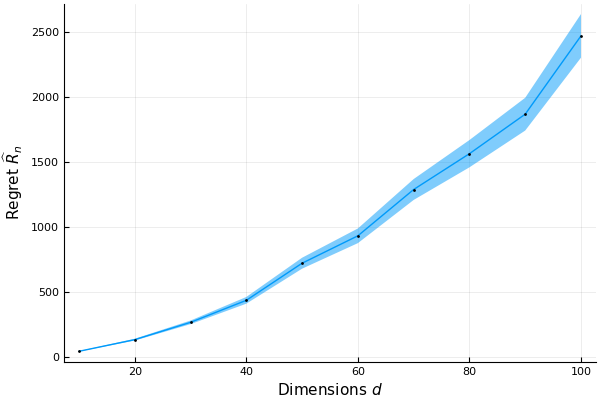
\includegraphics[scale=0.4]{dim-regret.png}
        \caption{Pseudo-regret as a function of the dimension\label{fig:regret_dim}}
    \end{subfigure}
    \begin{subfigure}[h]{0.45\textwidth}
        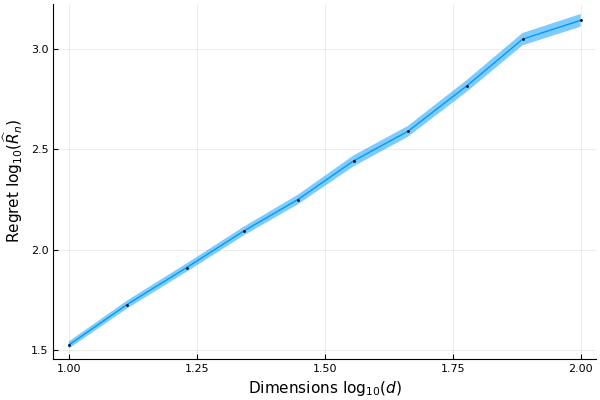
\includegraphics[scale=0.4]{dim-regret-logspace.png}
        \caption{\label{fig:regret_dim_logscale}Pseudo-regret as a function of the dimension}      
    \end{subfigure}
\end{figure}

\section{Privacy Proofs}
\label{apx_sec:privacy_proofs}

Before giving the omitted proofs from the body of the paper, we wish to have a short comparison between the regret bounds we get with the two different techniques to introduce differential privacy. In particular, omitting dependencies on any parameter but $n,d$ and $\varepsilon$, we have that the pseudo-regret bound of the Wishart noise (Corollary~\ref{cor:regret_with_Wishart}) is $\tilde O(\sqrt n(d+\tfrac{\sqrt d}\varepsilon))$; and that pseudo-regret bound of the Gaussian noise (Corollary~\ref{cor:regret_with_Gaussian}) is $\tilde O(\sqrt nd/\varepsilon)$. Before explaining how it came to be that the former has a better dependency on $\varepsilon$ than the latter, we first emphasize that (1) these bounds are only asymptotic (Wishart noise has far worst constants than the constants in the Gaussian bound), and that (2) this is an over simplification, as the many parameters of the problem may affect the regret bounds in favor of the Gaussian noise.

So, how come with Gaussian noise we get a worse dependency on $\varepsilon$ than in the Wishart case? The reason lies in the two factors. First, the degrees of freedom $k$ in the Wishart noise are of the form $k=d+O(\varepsilon^{-2})$, making the top eigenvalue of the added noise $\|\vec H_t\|$ proportional to $O(\sqrt{\log(n)k}+\sqrt d) = O(\sqrt{d\log(n)}+ \tfrac{\sqrt{\log(n)}}{\varepsilon})$, so we get an additive relation rather than a multiplicative relation. In contrast, sampling a Gaussian noise, even though the variance in each coordinate is $O(\log(n)\cdot \varepsilon^{-2})$ and independent of $d$, the bound on the noise in this case is greater by a factor of $\sqrt{d}$, resultsing in the bound $\|\vec H_t\| = O(\sqrt{d\log(n)}/\varepsilon)$. Second, the bound on $\gamma$ is different in the two cases. For Wishart noise, we are able to use the special structure of $\vec H_t$ being the Gram matrix of multivariate Gaussian samples to infer the $\|\vec h_t\|_{\inv{\vec H_t}}$ is basically a projection of a sample from a spherical Gaussian onto a $d$-dimensional space~--- making the bound $\gamma$ \emph{independent} of $mk$ (the degrees of freedom in the Wishart noise) and depends solely on $d$. As a result, $\gamma \ll \rho_{\max}$ in the Wishart noise case, and we have already established that $\rho_{\max}$ has additive dependencies between $\sqrt d$ and $\varepsilon^{-1}$. In contrast, we are unable to leverage on any structure in the Gaussian noise case, making our $\gamma$ bound very similar to $\rho_{\max}$ which is in this case $O(\sqrt d/\varepsilon)$.

Admittedly, we do not know if this is merely an artifact of our analysis, or rather truly a difference in the bound. It is possible that slightly revising the proof of Theorem~\ref{thm:linucb-regret} could leads to different bounds, which are identical between the two privacy-preserving techniques. To attempt to test this empirically requires ridicolously large $d$ and $1/\varepsilon$, which is far beyond what we could handle.

We now turn to providing the missing proofs from the main body of the paper. First, we give the omitted proof from Section~\ref{sec:dp-wishart}.

\PropWishartTails*
\begin{proof}
Seeing as $\vec H_t\sim\Wishart_d(\tilde L^2 \Eye, mk)$, straight-forward bounds on the eigenvalues of the Wishart distribution (e.g.~\cite{SheffetPrivateApproxRegression2015}, Lemma~A.3) give that w.p. $\geq 1- \tfrac \alpha{2n}$ all of the eigen values of $\vec H_t$ lie in the interval $\tilde L^2 \paren*{\sqrt{mk} \pm \paren*{\sqrt{d} + \sqrt{2\ln(\nicefrac{8n}{\alpha})}}}^2$. To estimate $\|\vec h_t\|_{\vec H_t^{-1}}$ we draw back to the definition of the Wishart distribution as the Gram matrix of samples from a multivariate Gaussian $\Normal(\vec 0, \tilde L^2\Eye)$. Denote this matrix of Gaussians as $[\vec Z ; \vec z]$ where $\vec Z\in \Real^{mk\times d}$ and $\vec z \in \Real^{mk}$, and we have that $\vec H_t = \transp{\vec Z} \vec Z$ and $\vec h_t = \transp{\vec Z} \vec z$, thus $\|\vec h_t\|_{\vec H_t^{-1}} = \sqrt{ \transp{\vec z} \vec Z (\transp{\vec  Z} \vec Z)^{-1}  \transp{\vec Z} \vec z }$. The matrix $\vec Z (\transp{\vec Z} \vec Z)^{-1}  \transp{\vec Z}$ is a projection matrix onto a $d$-dimensional space, and projecting the spherical Gaussian $\vec z$ onto this subspace results in a $d$-dimensional sphrical Gaussian. Using concentration bounds on the $\chi^2$-distribution~\ref{claim:chi2-tails} we have that w.p. $\geq 1- \tfrac \alpha{2n}$ it holds that $\|\vec h_t\|_{\vec H_t^{-1}}\leq \tilde L(\sqrt{d} + \sqrt{2\ln(\tfrac{2n}{\alpha})})$. %Taking a union bound over all $n$ days concludes the proof.
\end{proof}

\begin{theorem}[{\citealp[Theorem~4.1]{SheffetPrivateApproxRegression2015}}]%
  \label{thm:wishart-dp}%
  Fix $\varepsilon\in(0,1)$ and $\delta\in(0,1/e)$.  Let
  $A\in\Real^{n\times p}$ be a matrix whose rows have $l_2$-norm
  bounded by $\tilde L$.  Let $W$ be a matrix sampled from the
  $d$-dimensional Wishart distribution with $k$ degrees of freedom
  using the scale matrix $\tilde L^2\Eye{p}$ (i.e.\
  $W \sim \Wishart_p(\tilde L^2\Eye{p}, k)$) for
  $k \ge p + \floor[\big]{\frac{14}{\varepsilon^2}\cdot 2\log(4/\delta)}$.
  Then outputting $\XtX{A} + N$ is
  $(\varepsilon,\delta)$-differentially private with respect to
  changing a single row of $A$.
\end{theorem}

We now give the proof of the lower bound of any private algorithm under the stadard notion of differential privacy under continual observation, as discussed in Section~\ref{sec:lower_bounds}. First, of course, we need to define this notion. \DPDefinition
~We now prove the following.
\clmLinearRegretDP*
\DPLowerBoundProof





%%%%%%%%%%%%%%%%%%%%%%%%%%%%%%%%%%%%%%%%%%%%%%%%%%%%%%%%%%%%%%%%%%%%%%%%%%%
\cleardoublepage
\phantomsection
\addcontentsline{toc}{chapter}{Graveyard}
\todo[inline]{Remove following material from final version.}

\section{Ellipsoidal Confidence Sets}
\label{sec:ellips-conf-bounds}

Throughout this section we will fix some particular round $t \le n$
and suppress the subscripted $t$.

We will consider confidence sets for the value of $\theta^*$ that are
ellipsoidal with centre $\hat{\theta}$, of the form
$\set{\theta\in\Real^d \given \norm{V}{\theta-\hat{\theta}}^2 \le
  \beta}$.  Then the upper confidence bound of an action $x$ is
\begin{align*}
  \UCB(x) &= \max_{\theta: \norm{V}{\theta-\hat\theta}^2 \le \beta} \innerp{x}{\theta}
\end{align*}
We solve this constrained optimization problem by the method of
Lagrange multipliers:
\begin{align*}
  \mathcal{L}(\theta, \lambda) &= \innerp{x}{\theta} - \lambda(\norm{V}{\theta-\hat\theta}^2 - \beta) \\
  \nabla_\theta\mathcal{L}(\theta, \lambda) &= \transp{x} - \lambda\transp{(\theta-\hat\theta)}V = 0 \\
  \theta &= \hat\theta + \frac{{\inv{V}x}}{\lambda}
  \shortintertext{To find $\lambda$:}
  \beta &= \norm{V}{\theta-\hat\theta}^2
          = \norm[\bigg]{V}{\frac{\inv{V}x}{\lambda}}^2
          = \frac{1}{\lambda^2}\transp{x}\inv{V}x \\
  \lambda &= \norm{\inv{V}}{x} / \sqrt\beta
  \intertext{Which we substitute into the expression above:}
  \UCB(x) &= \innerp[\bigg]{x}{\hat\theta + \frac{\sqrt\beta}{\norm{\inv{V}}{x}}\inv{V}x} \\
          &= \innerp{x}{\hat\theta} + \sqrt\beta \norm{\inv{V}}{x}.
\end{align*}
We have therefore shown that if we construct an ellipsoidal confidence
set with an appropriate $V$ and $\beta$, then the requirements of
\cref{thm:linucb-regret} will be satisfied with the above $\UCB$
index.

Let $X_s \in \Real^d$ be the action vector selected by the algorithm at
time $s$, so that $X$ is a $t \times d$ matrix.  The \emph{Gram matrix} is given by
$G \defeq \transp{X}X \in \Real^{d \times d}$.  Let $y_s$ be the
reward received at time $s$, so that $y\in\Real^t$.

We will take $\hat{\theta}$ to be a regularized solution of the
least-squares system
\begin{align*}
  X\theta &\approx y,
\end{align*}
regularized by the symmetric positive definite matrix $H \succeq 0$:
\begin{align*}
  \hat{\theta} &= \argmin_\theta \frac{1}{2}\norm{}{X\theta - y}^2 + \frac{1}{2}\norm{H}{\theta}^2 \\
               &= \inv{\paren{\transp{X}X + H}} \transp{X}y \\
               &= \inv{\paren{\transp{X}X + H}} \transp{X} \paren{X\theta^* + \eta} \\
               &= \theta^* + \inv{\paren{\transp{X}X + H}}\paren{\transp{X}\eta - H\theta^*} \\
               &= \theta^* + \inv{V}Z - \inv{V}H\theta^*
\end{align*}
where we used the fact that $y = X\theta^* + \eta$ (and $\eta_s$ is the
noise in the reward at round $s$) and we defined $V \defeq \transp{X}X
+ H$ and $Z\defeq X^T\eta$.

\begin{lemma}\label{lemma:subgaussian-z}
  Under \cref{assumption:subgaussian-noise} and for any
$\lambda\in\Real^d$, the random variable $Z = \transp{X}\eta$ satisfies
  \begin{align*}
    \Ex{\exp(\transp{\lambda}Z)} \le \exp\paren{\norm{G}{\lambda}^2/2}.
  \end{align*}

  \begin{proof}
    We have
    \begin{align*}
      \Ex{\exp(\transp{\lambda}Z)}
      &= \Ex{\exp(\transp{\lambda}\transp{X}\eta)} \\
      &= \Ex[\Big]{\Ex[\Big]{\prod_{s=1}^t \exp\paren{\transp{\lambda}X_s\eta_s} \given \mathcal{F}_t}} \\
      &= \Ex[\Big]{\Ex[\Big]{\exp\paren{\transp{\lambda}X_t\eta_t} \given \mathcal{F}_t} \prod_{s=1}^{t-1} \exp\paren{\transp{\lambda}X_s\eta_s}} \\
      &\le \Ex[\Big]{\exp\paren{{(\transp{\lambda}X_t)}^2/2}
        \prod_{s=1}^{t-1} \exp\paren{\transp{\lambda}X_s\eta_s}}
      &\text{since $\eta_t$ is conditionally 1-subgaussian given $\mathcal{F}_t$}\\
      &\le \Ex[\Big]{\prod_{s=1}^t\exp({(\transp{\lambda}X_s)}^2/2)}
      &\text{similarly conditioning on $\mathcal{F}_{t-1},\mathcal{F}_{t-2},\dotsc$}\\
      &= \Ex[\Big]{\exp\paren[\Big]{\sum_{s=1}^t\frac{\transp{\lambda}X_s\transp{X_s}\lambda}{2}}} \\
      &= \exp\paren[\Big]{\frac{1}{2}\transp{\lambda}\transp{X}X\lambda}
        = \exp(\norm{G}{\lambda}^2/2)
      &\qedhere
    \end{align*}
  \end{proof}
\end{lemma}


\begin{lemma}\label{lemma:z-norm-bounded-whp}
  Suppose for any $\lambda\in\Real^d$ the random variable
  $Z=\transp{X}\eta$ satisfies
  $\Ex{\exp(\transp{\lambda}Z)} \le \exp(\norm{G}{\lambda}^2/2)$ (see,
  for example, \cref{lemma:subgaussian-z}).  Let
  $0 \prec H \in \Real^{d\times d}$ be any symmetric positive definite
  matrix.  Then for any $0 < \delta \le 1$, we have
  \begin{align*}
    \Prob[\Bigg]{\norm{\inv{(G+H)}}{Z} \ge \sqrt{2\log\frac{1}{\delta} + \log\frac{\det(G+H)}{\det H}}} &\le \delta.
  \end{align*}

  \begin{proof}
    We define
    \begin{align*}
      M_\lambda &\defeq \exp\paren[\Big]{\transp{\lambda}Z - \frac{1}{2}\transp{\lambda}G\lambda}.
    \end{align*}
    Now consider $\lambda\sim\mathcal{N}(0, \inv{H})$ to be a random
    variable with the density function $h(\lambda)$.  Define
    \begin{align*}
      \bar{M}
      &\defeq \int M_\lambda \,h(\lambda)\,d\lambda \\
      &= \frac{1}{\sqrt{{(2\pi)}^d \det\inv{H}}} \int\exp\paren[\Big]{\transp{\lambda}Z
        - \frac{1}{2}\transp{\lambda}G\lambda
        - \frac{1}{2}\transp{\lambda}H\lambda
        } \,d\lambda.
    \end{align*}
    We complete the square in the integrand:
    \begin{align*}
      \transp{\lambda}Z - \frac{1}{2}\transp{\lambda}G\lambda - \frac{1}{2}\transp{\lambda}H\lambda
      &= \frac{1}{2}\transp{Z}\inv{(G+H)}Z - \frac{1}{2}\transp{(\lambda - \inv{(G+H)}Z)}(G+H)(\lambda-\inv{(G+H)}Z) \\
      &= \frac{1}{2} \norm{\inv{(G+H)}}{Z}^2 - \frac{1}{2}\norm{G+H}{\lambda-\inv{(G+H)}Z}^2
    \end{align*}
    which we substitute into the previous equation to get
    \begin{align*}
      \bar{M}
      &= \frac{\exp\paren[\big]{\frac{1}{2} \norm{\inv{(G+H)}}{Z}^2}}{\sqrt{{(2\pi)}^d \det\inv{H}}}
        \int \exp\paren[\Big]{-\frac{1}{2} \norm{G+H}{\lambda-\inv{(G+H)}Z}^2} \,d\lambda \\
      &= \sqrt{\frac{\det H}{\det(G+H)}} \exp\paren[\Big]{\frac{1}{2}\norm{\inv{(G+H)}}{Z}^2}, \\
      \log\bar{M} &= \frac{1}{2}\norm{\inv{(G+H)}}{Z}^2 + \frac{1}{2}\log\frac{\det H}{\det(G+H)}.
    \end{align*}
    Our assumption gives us
    \begin{align*}
      \Ex{\exp(\transp{\lambda}Z)} &\le \exp\paren[\Big]{\frac{1}{2}\transp{\lambda}G\lambda} \\
      \Ex[\bigg]{\frac{\exp(\transp{\lambda}Z)}{\exp(\frac{1}{2}\transp{\lambda}G\lambda)}}
      &= \Ex{M_\lambda} \le 1, &\text{for all }\lambda\in\Real^d.
    \end{align*}
    Now, by Fubini's theorem we can exchange the expectation with the
    integral over $\lambda$:
    \begin{align*}
      \Ex{\bar{M}} &= \Ex[\Big]{\int M_\lambda\,h(\lambda)\,d\lambda} = \int \Ex{M_\lambda} \,h(\lambda)\,d\lambda \le 1
    \end{align*}
    and use a Chernoff bound:
    \begin{align*}
      \Prob{\log(\bar{M}) \ge u} &\le \exp(-u) \\
      \Prob[\Big]{\frac{1}{2}\norm{\inv{(G+H)}}{Z}^2 \ge u + \frac{1}{2}\log\frac{\det(G+H)}{\det H}} &\le \exp(-u) \\
      \Prob[\Big]{\norm{\inv{(G+H)}}{Z} \ge \sqrt{2u + \log\frac{\det(G+H)}{\det H}}} &\le \exp(-u).
    \end{align*}
    Substituting $u = \log(1/\delta)$ completes the proof.
  \end{proof}

\end{lemma}

%===============================================================================
% \hrule

% We see that
% \begin{align*}
%   \max_{\lambda\in\Real^d} \exp\paren[\Big]{\transp{\lambda}Z - \frac{1}{2}\transp{\lambda}G\lambda}
%   &= \exp\paren[\Big]{\max_{\lambda\in\Real^d} \transp{\lambda}Z - \frac{1}{2}\transp{\lambda}G\lambda}.
% \end{align*}
% The maximizer of this expression is given by taking the gradient and
% setting it to zero:
% \begin{align*}
%   \nabla_\lambda\brck[\Big]{\transp{\lambda}Z - \frac{1}{2}\transp{\lambda}G\lambda}_{\lambda=\lambda^*} = Z - G\lambda^* &= 0 \\
%   \lambda^* &= \inv{G}Z
% \end{align*}
% and thus
% \begin{align*}
%   \max_{\lambda\in\Real^d} \exp\paren[\Big]{\transp{\lambda}Z - \frac{1}{2}\transp{\lambda}G\lambda}
%   &= \exp\paren[\Big]{\transp{Z}\inv{G}Z - \frac{1}{2}\transp{Z}\inv{G}Z} \\
%   &= \exp\paren[\Big]{\frac{1}{2}\norm{\inv{G}}{Z}^2}.
% \end{align*}
% We define
% \begin{align*}
%   M_\lambda \defeq \exp\paren[\Big]{\transp{\lambda}Z - \frac{1}{2}\transp{\lambda}G\lambda}
% \end{align*}
% and use Chernoff's bound:
% \begin{align*}
%   \Pr\paren[\Big]{\frac{1}{2}\norm{\inv{G}}{Z}^2 > u}
%   &= \Pr\paren[\Big]{\max_{\lambda\in\Real^d}M_\lambda > u} \\
%   &\le \exp(-u) \Ex[\Big]{\max_{\lambda\in\Real^d} M_\lambda}.
% \end{align*}
% \hrule
%===============================================================================

\subsection{Ridge Regression}
\label{sec:ridge-regression}

We will now instantiate a concrete algorithm based on \emph{ridge
  regression}, i.e.\ using the regularizer $H=\rho I$ for some
$\rho>0$.  Thus we will have
\begin{align*}
  V_t &\defeq \rho I + \sum_{s=1}^t X_s\transp{X_s}
  \shortintertext{and}
  \hat{\theta}_t - \theta^* &= \inv{V_t}Z_t - \inv{V_t}H\theta^* \\
                          &= \inv{V_t}Z_t - \rho\inv{V_t}\theta^* \\
  V_t^{1/2}(\hat{\theta}_t - \theta^*) &= V_t^{-1/2}Z - \rho V_t^{-1/2}\theta^* \\
  \norm{V_t}{\hat{\theta}_t - \theta^*} &= \norm{}{V_t^{-1/2}Z - \rho V_t^{-1/2}\theta^*} \\
  &\le \norm{\inv{V_t}}{Z} + \rho\norm{\inv{V_t}}{\theta^*}.\
                          &\text{Triangle inequality} \\
  &\le \norm{\inv{V_t}}{Z} + \sqrt\rho \norm{}{\theta^*} &\text{Since } V_t \succeq \rho I.
\end{align*}
We now use \cref{lemma:subgaussian-z,lemma:z-norm-bounded-whp} in our
confidence bound:
\begin{align*}
  \Prob[\Bigg]{\norm{V_t}{\hat{\theta}_t - \theta^*} > \sqrt\rho\norm{}{\theta^*} + \sqrt{2\log\frac{1}{\delta} + \log\frac{\det V_t}{\det \rho I}}}
  &\le \delta.
\end{align*}
We assume that $\norm{}{\theta^*} \le S$.  We use the union bound,
replacing $\delta$ with $\delta/n$ to get a bound that holds uniformly
at every round:
\begin{align*}
  \sqrt{\beta_t} &= \sqrt\rho S + \sqrt{2\log\frac{n}{\delta} + \log\frac{\det V_t}{\det \rho I}}.
\end{align*}
Applying \cref{thm:linucb-regret} gives us the regret bound
\begin{align*}
  \widehat{R}_n
  &\le \sqrt{8dn\beta_{n-1}\log\frac{\tr V_0 + nL^2}{d\det^{1/d} V_0}}
    = \sqrt{8dn\beta_{n-1}\log\frac{d\rho + nL^2}{d\rho}}
  \shortintertext{where}
  \sqrt{\beta_{n-1}}
  &= \sqrt\rho S + \sqrt{2\log\frac{n}{\delta} + \log\frac{\det V_{n-1}}{\det \rho I}} \\
  &\le \sqrt\rho S + \sqrt{2\log\frac{n}{\delta} + d\log\paren*{1 + \frac{nL^2}{d\rho}}}.
\end{align*}
Choosing $\delta=1/n$ and constant $\rho$ gives $\sqrt{\beta_{n-1}} =
O(d^{1/2}\log^{1/2}(n/d))$ and thus the expected regret of Linear UCB
with ellipsoidal confidence sets satisfies
\begin{align*}
  \widehat{R}_n &= O(\beta_n^{1/2}\sqrt{dn\log(n/d)}) = O(d\log(n/d)\sqrt{n}).
\end{align*}




% \section{Facts About Random Variables}

% \begin{definition}[Subgaussian random variable]\label{def:subG}
%   A real-valued random variable $X$ is \emph{$\sigma^2$-subgaussian}
%   if its moment-generating function satisfies:
%   \begin{align*}
%     \mgf_X(s) \defeq \Ex{\exp(sX)} &\le \exp(s^2\sigma^2/2).
%   \end{align*}
% \end{definition}

% \begin{definition}[Subexponential random variable]\label{def:subExp}
%   A real-valued random variable $X$ is \emph{$\lambda$-subexponential}
%   if its moment-generating function satisfies:
%   \begin{align*}
%     \mgf_X(s) \defeq \Ex{\exp(sX)} &\le \exp(s^2\lambda^2/2),
%     &\text{for all } \abs{s}\le 1/\lambda.
%   \end{align*}
% \end{definition}

% \begin{definition}[Subgaussian/subexponential random vector]
%   A random vector $X\in\Real^b$ is subgaussian (subexponential) if the
%   random variable $\innerp{v}{X}$ is subgaussian (subexponential) for
%   any $v\in\Real^n$ with $\norm{}{v}=1$.
% \end{definition}

% \begin{definition}[Subgaussian/subexponential random matrix]
%   A random matrix $W\in\Real^{n\times m}$ is subgaussian (subexponential)
%   if the random vector $Wu\in\Real^n$ is subgaussian
%   (subexponential) for any $u\in\Real^m$ with $\norm{}{u}=1$.
% \end{definition}

\section{Other Proofs}

\begin{lemma}[{\citealp[Lemma~9]{AbbasiYadkoriImprovedAlgorithmsLinear2011}}]\label{lemma:martingale-mgf}
  Let $X_1, X_2, \dotsc \in \Real$ and
  $\sigma_1, \sigma_2, \dotsc \in \Real$ be sequences of random
  variables and let
  $\mathcal{F}_1 \subset \mathcal{F}_2 \subset \dotsb$ be a
  filtration.  Suppose that each $X_t \in \mathcal{F}_t$ and almost
  surely
  $\Ex{\exp(\lambda X_t)\given \mathcal{F}_{t-1}} \le
  \exp(\sigma_t^2\lambda^2/2)$ (i.e. each
  $\sigma_t \in \mathcal{F}_{t-1}$ and $X_t$ is conditionally
  $\sigma_t$-subgaussian given $\mathcal{F}_{t-1}$).  For any
  $\lambda\in\Real$, define
  \begin{align*}
    M_{t,\psi} &\defeq \exp\paren[\bigg]{\sum_{s=1}^t \psi X_s - \frac{1}{2}\sigma_s^2\psi^2}.
  \end{align*}
  Let $\tau$ be a stopping time with respect to
  ${(\mathcal{F}_t)}_{t=1}^\infty$.  Then $M_{\tau,\psi}$ is almost surely
  well-defined and $\Ex{M_{\tau,\psi}} \le 1$.

  \begin{proof}
    We will show that ${(M_{t,\psi})}_{t=1}^\infty$ is a
    supermartingale.  Let
    \begin{align*}
      D_{t,\psi} &\defeq \exp\paren[\bigg]{\psi X_t - \frac{1}{2}\sigma_t^2\psi^2}.
    \end{align*}
    By the conditional subgaussianity of $X_t$, we have
    \begin{align*}
      \Ex{D_{t,\psi}\given\mathcal{F}_{t-1}}
      &= \Ex{\exp(\psi X_t)\given\mathcal{F}_{t-1}}
        \cdot \exp\paren[\bigg]{-\frac{1}{2}\sigma_t^2\psi^2}
      \le \exp\paren[\bigg]{\frac{1}{2}\sigma_t^2\psi^2}
        \cdot \exp\paren[\bigg]{-\frac{1}{2}\sigma_t^2\psi^2}
      = 1.
    \end{align*}
    It is also clear that $D_{t,\psi}$ is $\mathcal{F}_t$-measurable
    (since $X_t,\sigma_t \in \mathcal{F}_t$), and therefore so is
    $M_{t,\psi}$.  Furthermore,
    \begin{align*}
      \Ex{M_{t,\psi}\given\mathcal{F}_{t-1}}
      &= \Ex{M_{t-1,\psi}\cdot D_{t,\psi}\given\mathcal{F}_{t-1}}
        = M_{t-1,\psi} \Ex{D_{t,\psi}\given\mathcal{F}_{t-1}}
        \le M_{t-1,\psi},
    \end{align*}
    showing that $M_{t,\psi}$ is indeed a supermartingale and therefore
    by Doob's optional stopping theorem
    $\Ex{M_{\tau,\psi}} \le \Ex{M_{0,\psi}} = 1$.

    Now, we argue that $M_{\tau,\psi}$ is well-defined.  By the
    convergence theorem for non-negative supermartingales,
    $M_{\infty,\psi} = \lim_{t\to\infty}M_{t,\psi}$ is almost surely
    well-defined.  Hence, $M_{\tau,\psi}$ is almost surely
    well-defined independently of whether $\tau<\infty$ holds or not.
    Next, we show that $\Ex{M_{\tau,\psi}} \le 1$.  For this, let
    $Q_{t,\psi} \defeq M_{\min\{\tau,t\},\psi}$ be a stopped
    version of ${(M_{t,\psi})}_t$.  By Fatou's lemma,
    $\Ex{M_{\tau,\psi}} = \Ex{\liminf_{t\to\infty}Q_{t,\psi}} \le
    \liminf_{t\to\infty}\Ex{Q_{t,\psi}} \le 1$, showing the
    $\Ex{M_{\tau,\psi}} \le 1$ indeed holds.
  \end{proof}
\end{lemma}

\begin{lemma}
  Let $n\in\Nat$ and $\varepsilon>0$ and $\sigma^2>0$.  Let
  $X_1,X_2,\dotsc,X_n\in\Real$ and
  $\sigma_1,\sigma_2,\dotsc,\sigma_n\in\Real$ be sequences of random
  variables and let
  $\mathcal{F}_1 \subset \mathcal{F}_2 \subset \dotsb \subset
  \mathcal{F}_n$ be a filtration.  Suppose that each
  $X_t\in\mathcal{F}_t$ and almost surely each $\sigma_t \le \sigma$
  and each $X_t$ is conditionally $\sigma_t$-subgaussian given
  $\mathcal{F}_{t-1}$.  Then
  \begin{align*}
    \Prob[\Big]{\exists t \le n. \sum_{s=1}^t X_s \ge
    \sqrt{2\gamma_nV_t\log(N/\delta)}}
    &\le \delta,
  \end{align*}
  where
  \begin{align*}
    V_t &\defeq \max\set[\Big]{\varepsilon,\sum_{s=1}^t \sigma_s^2}, &
    \gamma_n &\defeq 1 + \frac{1}{\log(n)}, &
    N &\defeq 1 + \ceil*{\frac{\log(n\sigma^2/\varepsilon)}{\log(\gamma_n)}}.
  \end{align*}

  \begin{proof}
    For $\psi\in\Real$ define
    \begin{align*}
      M_{t,\psi} &\defeq \exp\paren[\bigg]{\sum_{s=1}^t \psi X_s - \frac{1}{2}\psi^2\sigma_s^2}.
    \end{align*}
    If $\tau \le n$ is a stopping time with respect to $\mathcal{F}$,
    then $\Ex{M_{\tau,\psi}} \le 1$ by \cref{lemma:martingale-mgf}.
    Therefore by Markov's inequality,
    \begin{align*}
      \delta/N
      &\ge \Prob{M_{\tau,\psi} \ge N/\delta} \\
      &= \Prob[\bigg]{\exp\paren[\Big]{\sum_{s=1}^\tau \psi X_s - \frac{\psi^2\sigma_s^2}{2}} \ge N/\delta} \\
      &= \Prob[\bigg]{\psi \sum_{s=1}^\tau X_s - \frac{\psi\sigma_s^2}{2} \ge \log(N/\delta)} \\
      &\ge \Prob[\bigg]{\sum_{s=1}^\tau X_s \ge \frac{\log(N/\delta)}{\psi} + \frac{\psi V_\tau}{2}},
      &\text{since } V_\tau \ge \sum_{s=1}^\tau \sigma_s^2.
    \end{align*}
    To get the tightest tail bound, we want to minimize the quantity
    on the right side of the inequality; it attains a minimum of
    $\sqrt{2V_\tau \log(1/\delta)}$ at
    $\psi_{\min} \defeq \sqrt{2\log(N/\delta)/V_\tau}$.  Furthermore,
    for any $\psi\ge\psi_{\min}$ that quantity is at most
    $\psi V_\tau$.

    However, since $V_\tau$ is a random quantity, we cannot simply set
    $\psi \defeq \psi_{\min}$.  Instead, we recognize that
    $V_\tau \in [\varepsilon, n\sigma^2]$ almost surely, and we can
    logarithmically cover this range with the $N$ values
    $\varepsilon\gamma_n^{k-1}$ for $k=1,2,\dotsc,N$; at least one of
    these must lie in the interval $[V_\tau/\gamma_n, V_\tau]$.  Then
    we can define the corresponding values
    \begin{align*}
      \psi_k &\defeq \sqrt{\frac{2\log(N/\delta)}{\varepsilon\gamma_n^{k-1}}},
              &\text{for } k=1,2,\dotsc,N;
    \end{align*}
    there must be some value of $k$ for which
    $\psi_k \in [\psi_{\min}, \gamma_n\psi_{\min}]$.  Using a union bound
    over these $N$ values, we get
    \begin{align*}
      \delta
      &\ge \Prob[\bigg]{\exists k\in[N]. \sum_{s=1}^\tau X_s \ge \frac{\log(N/\delta)}{\psi_k} + \frac{\psi_k V_\tau}{2}} \\
      &\ge \Prob[\bigg]{\sum_{s=1}^\tau X_s \ge \gamma_n\psi_{\min}V_\tau} \\
      &= \Prob[\bigg]{\sum_{s=1}^\tau X_s \ge \sqrt{2\gamma_nV_\tau\log(N/\delta)}}.
    \end{align*}
    To complete the proof, define the stopping time $\tau =
    \min\set{n,\tau_n}$ where
    \begin{align*}
      \tau_n &\defeq \min\set[\Big]{t \le n \given \sum_{s=1}^tX_s \ge \sqrt{2\gamma_nV_t\log(N/\delta)}}.
              \qedhere
    \end{align*}
  \end{proof}
\end{lemma}


\end{document}

%%% Local Variables:
%%% mode: latex
%%% TeX-master: t
%%% End:
